\documentclass[hyperref={unicode}, xcolor={svgnames, table},
usepdftitle=false]{beamer}

\usetheme{Boadilla}
\usecolortheme{beaver}
\usefonttheme{serif}
\setbeamercovered{dynamic}

\setbeamertemplate{enumerate items}[square]
\setbeamertemplate{navigation symbols}{}

\usepackage[T2A]{fontenc}
\usepackage[utf8]{inputenc}

\usepackage[macedonian]{babel}
\usepackage[babel]{microtype}

\usepackage{mathtools, amssymb, amsthm, centernot}

\usepackage{graphicx, caption, subcaption}

\usepackage{booktabs, array, multicol}
\usepackage[newfloat]{minted}

\usepackage{csquotes}

\usepackage[os=win]{menukeys}
\usepackage{tikz}

\usepackage{siunitx}
\sisetup{%
  detect-all,
  round-mode=places,
  round-precision=2,
  group-separator=.,
  output-decimal-marker={,}
}

\deftranslation[to=macedonian]{Theorem}{Теорема}
\deftranslation[to=macedonian]{theorem}{теорема}
\deftranslation[to=macedonian]{Definition}{Дефиниција}
\deftranslation[to=macedonian]{definition}{дефиниција}

\DeclareMathOperator*{\argmax}{arg\,max}
\DeclareMathOperator*{\argmin}{arg\,min}

\graphicspath{{Figures/}}

\hypersetup{%
  pdfinfo={%
    Title={Вовед во R},
    Subject={Статистика},
    Author={Дарио Ѓорѓевски},
    Keywords={Статистика, Дескриптивни статистики, Визуелизација, Оценување на
      параметри, Генерирање на случајни броеви}
  }
}

\theoremstyle{remark}
\newtheorem*{remark}{Забелешка}

\title{Вовед во R}

\subtitle{Елементи од јазикот, работа со распределби, дескриптивни статистики,
  визуелизација, и оценување на параметри}

\author[Дарио Ѓорѓевски]{%
  Дарио Ѓорѓевски\inst{1}\\%
  \href{mailto:gjorgjevski.dario@students.finki.ukim.mk}%
  {\texttt{gjorgjevski.dario@students.finki.ukim.mk}}
}

\institute[ФИНКИ]{%
  \inst{1}Факултет за компјутерски науки и инженерство\\%
  Универзитет Св.\ Кирил и Методиј, Скопје
}

\date{\today}

\logo{
\includegraphics[height=0.66cm]{Logo.png}}

\AtBeginSection[]{%
  \begin{frame}{Содржина}
    \tableofcontents[currentsection, hideothersubsections]
  \end{frame}
}

\begin{document}

\begin{frame}
  \titlepage
\end{frame}

\section{Основни информации за R}
\begin{frame}{Што е R?}
  R е:
  \begin{itemize}
  \item Колекција софтверски алатки кои служат за:
    \begin{itemize}
    \item Читање на податоци и нивно манипулирање;
    \item Вршење пресметки;
    \item Статистичка анализа;
    \item Приказ на резултати.
    \end{itemize}
  \item Open-source верзија на програмскиот јазик S: јазик за манипулација на
    \emph{објекти};
  \item Платформа за развој и имплементација на (статистички) алгоритми.
  \end{itemize}

  R, заедно со пакети од имплементирани алгоритми и функционалности, може да
  бидат симнати од
  \href{https://cran.r-project.org/}{\texttt{cran.r-project.org}}.
\end{frame}

\begin{frame}{Интерактива сесија}{Читање команди}
  Со започнување на R, започнува и интерактивна сесија.  Корисниците внесуваат
  \emph{команди} во конзолата на R.  Кога R е спремен да прочита команда, печати
  prompt `\texttt{>}'.  Командите се состојат од \emph{изрази}.

  Изразите
  \begin{itemize}
  \item се одделени со точка-зарпика (\texttt{;}) или newline;
  \item може да бидат групирани во поголеми изрази, наречени \emph{блокови}, со
    употреба на \texttt{\{} и \texttt{\}}.
  \end{itemize}

  Коментари може да бидат вклучени со тараба (\texttt{\#}) и важат сѐ до крајот
  на редот.
\end{frame}

\begin{frame}[fragile]{Интерактивна сесија}{Евалуирање на команди}
  Корисникот внесува команда и истата ја евалуира со притискање на
  \keys{\return}.  Вредноста на командата се печати назад во конзолата; на пр.:
\begin{minted}{R}
> 2 + 2
[1] 4
>
\end{minted}

  Prompt-от `\texttt{>}' ни кажува дека R е спремен да вчита нова команда.
  Доколку внесена команда не е комплетна, prompt-от се променува во
  `\texttt{+}', и останува така сѐ до комплетирање на командата.
\end{frame}

\begin{frame}{Како работи R?}
  R е програмски јазик кој работи со \emph{објекти}.  Дури и променливите и
  функциите се објекти и истите може да бидат користени како било кој друг
  објект.
  \begin{itemize}
  \item Објектите се креираат во меморија и зачувуваат во датотека
    \texttt{.RData};
  \item Извршените команди се зачувуваат во датотека \texttt{.Rhistory}, и може
    да бидат изминати со \keys{\arrowkeyup} и \keys{\arrowkeydown};
  \item Лошите команди може да бидат прекинати со \keys{\esc} или
    \keys{\ctrl+C};
  \item Команди може да бидат зачувани во датотека со екстензија \texttt{.R} и
    евалуирани со \mintinline{R}{source(file, ...)};
  \item Сесијата се прекинува со повик на функцијата \mintinline{R}{q} или
    испраќање на \texttt{EOF} сигнал (\keys{\ctrl+D}).
  \end{itemize}
\end{frame}

\begin{frame}[fragile]{R како калкулатор}
  R може да извршува стандардни аритметички пресметки:
\begin{minted}[mathescape]{R}
> exp(-2)
[1] 0.1353353
> 2 * 3 * 4* 5
[1] 120
> pi  # R знае за бројот $\pi$
[1] 3.141593
> 1000 * (1 + 0.075)^2 - 1000
[1] 155.625
> sin(pi)
[1] 1.224647e-16  # $\num{1.224647e-16} \approx 0$
> 8 %/% 3 + 8 %% 5  # Целобројно делење и остаток
[1] 5
\end{minted}
\end{frame}

\begin{frame}[fragile]{Доделување вредности}
  Често сакаме одредени вредности да ги зачуваме во променливи.  За да ја
  доделиме вредноста \num{10} на симболот \mintinline{R}{x}, пишуваме
\begin{minted}{R}
> x <- 10
\end{minted}
  и притискаме \keys{\return}.

  Еквивалентно, можеме да ја искористиме функцијата
\begin{minted}{R}
> assign("x", 10)
\end{minted}

  Видлив резултат од извршената команда нема, но сега \mintinline{R}{x} има
  вредност \num{10} и може да се користи во понатамошни изрази:
\begin{minted}{R}
> x
[1] 10
> x + x
[1] 20
> sqrt(x)
[1] 3.162278
\end{minted}
\end{frame}

\begin{frame}{Case sensitivity и имиња на променливи}
  R е \emph{case sensitive}: \mintinline{R}{x} и \mintinline{R}{X} не се
  однесуваат на истиот објект.

  Идентификаторите
  \begin{itemize}
  \item може да содржат букви, цифри, долна црта (`\texttt{\_}'), и точка
    (`\texttt{.}');
  \item не смее да започнуваат со цифра, долна црта, или точка следена од цифра.
  \end{itemize}

  Некои имиња се резервирани од R и не може да бидат користени како
  идентификатори: \texttt{if else repeat while function}, ...
\end{frame}

\begin{frame}{Објекти}{Основни информации}
  Статистички анализи не е погодно да се вршат на едноставни броеви.  R работи
  така што креира \emph{објекти} користејќи различни функции за нивно креирање и
  манипулирање.
  \begin{itemize}
  \item Вектори од
    \begin{itemize}
    \item броеви;
    \item логички вредности;
    \item карактери (strings);
    \item комплексни броеви.
    \end{itemize}
  \item Матрици и \(n\)-димензионални низи;
  \item Листи: произволни колекции од објекти од било кој тип;
  \item Data frames: листи со правоаголна структура;
  \item Функции;
  \item Специјален објект \mintinline{R}{NULL}.
  \end{itemize}
\end{frame}

\begin{frame}[fragile]{Објекти}{Workspace (работна околина)}
  За време на една сесија, објектите се зачувуваат по име.  Функцијата
\begin{minted}{R}
> ls()
\end{minted}
  ги печати имињата на сите моментално зачувани објекти во \emph{workspace}-от
  (работната околина).  Објекти може да бидат отстранети со функцијата
\begin{minted}{R}
> rm(x)          # Избриши ја променливата x.
> rm(list=ls())  # Избриши ги сите објекти.
\end{minted}

  На крајот на секоја сесеија, корисникот е прашан дали состојбата на работната
  околина да биде зачувана во датотеката \texttt{.RData}.
\end{frame}

\section{Објекти и едноставни манипулации}

\begin{frame}[fragile]{Вектори}{Типови на вектори и функцијата
    \mintinline{R}{c}}
  Векторите се \emph{наједнсставен} тип на објект во R.  Постојат \num{4}
  основни типови на вектори:
  \begin{enumerate}
  \item Нумерички вектори;
  \item Вектори од карактери;
  \item Вектори од логички вредности;
  \item Вектори од комплексни броеви.
  \end{enumerate}

  За дефинирање на вектор \mintinline{R}{x} со броевите \num{10.4}, \num{5.6},
  \num{3.1}, \num{6.4}, и \num{21.7}, користиме
\begin{minted}{R}
> x <- c(10.4, 5.6, 3.1, 6.4, 21.7)
\end{minted}
\end{frame}

\begin{frame}[fragile]{Вектори}{Печатење и пристап до вредности}
  За да ја испечатиме содржината на \mintinline{R}{x} користиме
\begin{minted}{R}
> x
[1] 10.4 5.6 3.1 6.4 21.7
\end{minted}

  \mintinline{R}{[1]} на почетокот ни го кажува индексот на првиот елемент.
  Како што можеме да забележиме, R користи \num{1}-based indexing.

  Да пристапиме до елемент на дадена позиција користиме
\begin{minted}{R}
> x[1]
[1] 10.4
> x[5]
[1] 21.7
\end{minted}

  Со функцијата \mintinline{R}{c}
\begin{minted}{R}
> y <- c(x, 0, x)
\end{minted}
  можеме и да креираме две копии од \mintinline{R}{x} со \num{0} на средината.
\end{frame}

\begin{frame}[fragile]{Вектори}{Пресметки со нумерички вектори}
  \begin{itemize}
  \item Пресметките вообичаено се вршат по-компонентно:
\begin{minted}{R}
> 1 / x
[1] 0.09615385 0.17857143 0.32258065 0.15625000
[5] 0.04608295
\end{minted}
  \item Пократките вектори се „рециклираат“ да се совпаднат со подолгите:
\begin{minted}{R}
> x + c(1, 2)
[1] 11.4  7.6  4.1  8.4 22.7
Warning message:
In x + c(1, 2) :
  longer object length is not a multiple
  of shorter object length
\end{minted}
  \end{itemize}
\end{frame}

\begin{frame}[fragile]{Вектори}{Функции кои работат со нумерички вектори}
  \begin{itemize}
  \item Некои функции враќаат повеќе вредности---една за секој елемент на
    векторот (\mintinline{R}{sin}, \mintinline{R}{cos}, \mintinline{R}{round},
    \mintinline{R}{exp}, \mintinline{R}{log}, ...):
\begin{minted}{R}
> round(x)
[1] 10  6  3  6 22
\end{minted}
  \item Некои функции враќаат една вредност (\mintinline{R}{sum},
    \mintinline{R}{prod}, \mintinline{R}{length}, ...):
\begin{minted}{R}
> sum(x) + prod(x)
[1] 25121.15
\end{minted}
  \item Некои функции се „специјални“ (\mintinline{R}{sort},
    \mintinline{R}{cumsum}, \mintinline{R}{range}, ...)
  \end{itemize}
\end{frame}

\begin{frame}[fragile]{Вектори}{Вектори од комплексни броеви}
  Комплексните броеви се означуваат како \mintinline{R}{5 + 6i}.  Мора да
  внимаваме, R не го прави тоа автоматски за нас:
\begin{minted}{R}
> sqrt(-17)
[1] NaN
Warning message:
In sqrt(-17) : NaNs produced
> sqrt(-17 + 0i)
[1] 0+4.123106i
> log(-5 + 6i)  # Комплексен логаритам.
[1] 2.055437+2.265535i
\end{minted}
\end{frame}

\begin{frame}[fragile]{Вектори}{Генерирање на секвенци}
\begin{minted}{R}
> 1:10
 [1]  1  2  3  4  5  6  7  8  9 10
> seq(1, 10)  # Еквивалентно со погорното.
 [1]  1  2  3  4  5  6  7  8  9 10
> seq(1, 10, by=2)
[1] 1 3 5 7 9
> seq(1, 10, length=5)
[1]  1.00  3.25  5.50  7.75 10.00
> rep(x, 2)
 [1] 10.4  5.6  3.1  6.4  21.7 10.4  5.6  3.1  6.4 21.7
\end{minted}
\end{frame}

\begin{frame}[fragile]{Вектори}{Вектори од карактери}
  Вектор од карактери со должина \num{1} се добива со ставање на збор во двојни наводници:
\begin{minted}[mathescape]{R}
> # c1 ќе биде вектор од карактери со должина $\num{1}$
> c1 <- "Canberra"
\end{minted}

  Можеме пак да ја искористиме функцијата \mintinline{R}{c}:
\begin{minted}{R}
> c2 <- c(z, "Syndey", "Melbourne", "Newcastle"); c2
[1] "Canberra"  "Syndey"    "Melbourne" "Newcastle"

> c3 <- c("Perth", c2); c3
[1] "Perth"     "Canberra"  "Syndey"    "Melbourne"
[5] "Newcastle"
\end{minted}
\end{frame}

\begin{frame}[fragile]{Вектори}{Вектори од логички вредности}
  \begin{itemize}
  \item Вектор од логички вредности ги содржи вредностите \mintinline{R}{TRUE},
    \mintinline{R}{FALSE}, и \mintinline{R}{NA}
  \item Ваквите вектори се добиваат од \emph{условни изрази}:
\begin{minted}{R}
> temp <- x > 13
\end{minted}
    Овој израз го зема секој елемент од \mintinline{R}{x}, и го споредува со
    \num{13}.  Резултатот е логички вектор со истата должина како
    \mintinline{R}{x}, кој на позиција \(i\) ја има вредноста од споредбата
    \mintinline{R}{x[i] > 13}.
  \item Оператори \mintinline{R}{>}, \mintinline{R}{>=}, \mintinline{R}{<},
    \mintinline{R}{<=}, \mintinline{R}{==}, \mintinline{R}{!=},
    \mintinline{R}{&}, \mintinline{R}{|}, \mintinline{R}{&&},
    \mintinline{R}{||}.
  \item \mintinline{R}{&} и \mintinline{R}{|} враќаат вектори добиени
    по-компонентно, додека \mintinline{R}{&&} и \mintinline{R}{||} враќаат една
    вредност добиена од првите елементи.
  \end{itemize}
\end{frame}

\begin{frame}[fragile]{Вредности кои недостасуваат}
  Понекогаш точната вредност на одреден елемент во векторот не ја знаеме.
  Таквите вредности се претсавени со \mintinline{R}{NA}.

  Можеме да провериме дали некоја вредност е \mintinline{R}{NA} користејќи ја
  функцијата \mintinline{R}{is.na}:
\begin{minted}{R}
> is.na(x)
[1] FALSE FALSE FALSE FALSE FALSE
> w <- c(1:3, rep(NA, 2), 5)
> w
[1]  1  2  3 NA NA  5
> is.na(w)
[1] FALSE FALSE FALSE  TRUE  TRUE FALSE
\end{minted}
\end{frame}

\begin{frame}[fragile]{Вектори}{Индексирање}
  Веќе видовме како да индексираме вектори и да пристапиме до еден елемент.  На
  сличен начин можеме да пристапиме и до повеќе елементи истовремено, така што
  наместо со една ќе индексираме со повеќе вредности:
  \begin{itemize}
  \item
\begin{minted}{R}
> ex1 <- w[!is.na(w)]
\end{minted}
    ги зема елементите кои \emph{не} се \mintinline{R}{NA}.
  \item
\begin{minted}{R}
> ex2 <- w[1:3]
\end{minted}
    ги зема елементите на позиции \num{1}, \num{2}, и \num{3}.
\item
\begin{minted}{R}
> ex3 <- w[-c(1, 4)]
\end{minted}
  ги зема \emph{сите} елементи \emph{освен} тие на позиции \num{1} и \num{4}.
\end{itemize}
\end{frame}

\begin{frame}[fragile]{Вектори}{Модифицирање на вредности}
  Модифицирањето е исто како индексирањето, само што истовремено доделуваме
  вредност:
\begin{minted}[mathescape]{R}
# Првиот два елементи ќе имаат вредност $\num{5}$.
> x[1:2] <- 5
> x
[1]  5.0  5.0  3.1  6.4 21.7
> # Им додаваме $\num{5}$ на сите помали елементи.
> x[x < 5] <- x[x < 5] + 5
> x
[1]  5.0  5.0  8.1  6.4 21.7
\end{minted}
\end{frame}

\begin{frame}[fragile]{Фактори}{Основни информации}
  Факторите се специјални типови на податоци кои се користат за категорични
  податоци, на пр.: пол, социјален статус, боја на очи, и сл.
  \begin{itemize}
  \item Внатрешната репрезентација е како нумерички вектор со вредности
    \(1, 2, \ldots, k\), каде \(k\) е бројот на \emph{нивоа} во факторот;
  \item Може да бидат подредени или неподредени;
  \item Освен нумеричкиот вектор, факторот содржи и вектор од карактери кој го
    опишува секое ниво.
  \end{itemize}
\end{frame}

\begin{frame}[fragile]{Фактори}{Пример}
  Нека некоја анкета биде спроведена на \num{200} лица од машки и \num{300} лица
  од женски пол.  Најдобар начин да ги зачуваме половите е со користење на
  фактор:
\begin{minted}{R}
> gender <- c(rep("Male", 200), rep("Female", 300))
> gender <- factor(gender)
> levels(gender)
[1] "Female" "Male"
\end{minted}
  Внатре во R овој фактор е зачуван како
  \begin{table}[b]
    \centering
    \begin{tabular}{| c | c |}
      \hline
      1 & Female \\ \hline
      2 & Male \\
      \hline
    \end{tabular}
  \end{table}
\end{frame}

\begin{frame}[fragile]{Матрици}{Основни информации}
  Матрицата
  \begin{itemize}
  \item е дводимензионална низа од броеви;
  \item има редици и колони;
  \item е често користена во статистиката.
  \end{itemize}

  Во R матриците се претставуваат како вектори \emph{со димензии}.
\begin{minted}[mathescape]{R}
> m <- rnorm(12)     # Генерирај $\num{12}$ случајни броја.
> dim(m) <- c(3, 4)  # Подреди ги во $3 \times 4$ матрица.
> m
             [,1]       [,2]       [,3]      [,4]
[1,]  1.152181249  0.2933196 -0.7658679 -0.014726
[2,] -0.354144751  1.0523346  0.6052899 -1.080053
[3,]  0.003613231 -0.2068498 -2.5782982 -1.881613
\end{minted}
\end{frame}

\begin{frame}[fragile]{Матрици}{Функциите \mintinline{R}{dim} и \mintinline{R}{matrix}}
  Функцијата \mintinline{R}{dim} се користи за читање или промена на димензиите
  на објект.  Кога вектор има димензија \(m \times n\), R истиот го третира како
  матрица.

  Друг начин за креирање на матрици е со \mintinline{R}{matrix}:
\begin{minted}[mathescape]{R}
> n <- rnorm(10)  # Генерирај $\num{10}$ случајни броеви.
> matrix(n, nrow=5, ncol=2, byrow=TRUE)
            [,1]        [,2]
[1,] -0.05156321 -0.73200194
[2,]  0.75949863 -0.38434349
[3,]  1.22055333  0.41306536
[4,]  0.39608629  0.41769997
[5,]  0.47927784 -0.08826759
\end{minted}
\end{frame}

\begin{frame}[fragile]{Матрици}{Корисни функции}
  Аргументот \mintinline{R}{byrow=TRUE} му кажува на R да ја пополни матрицата
  редица по редица наместо колона по колона.

  Корисни функции за матрици се \mintinline{R}{nrow}, \mintinline{R}{ncol},
  \mintinline{R}{rownames}, и \mintinline{R}{colnames}.
\begin{minted}{R}
> nrow(m)
[1] 3
> rownames(m)
NULL
> rownames(m) <- c("A", "B", "C")
> m
          [,1]       [,2]       [,3]      [,4]
A  1.152181249  0.2933196 -0.7658679 -0.014726
B -0.354144751  1.0523346  0.6052899 -1.080053
C  0.003613231 -0.2068498 -2.5782982 -1.881613
\end{minted}
\end{frame}

\begin{frame}[fragile]{Матрици}{Транспонирање, додавање редици или колони}
  Функцијата \mintinline{R}{t} врши транспонирање:
\begin{minted}{R}
> t(m)
              A          B            C
[1,]  1.1521812 -0.3541448  0.003613231
[2,]  0.2933196  1.0523346 -0.206849760
[3,] -0.7658679  0.6052899 -2.578298206
[4,] -0.0147260 -1.0800535 -1.881613177
\end{minted}

  За спојување на вектори и матрици ги користиме функциите \mintinline{R}{rbind}
  (додавање редици) и \mintinline{R}{cbind} (додавање колони).  Доколку
  спојуваме матрици со матрици, димензиите на истите мора да се совпаѓаат.
  Доколку спојуваме вектори со било што, векторите се рециклираат или кратат сѐ
  додека не се добие соодветната димензија.
\end{frame}

\begin{frame}[fragile]{Матрици}{Пример со \mintinline{R}{rbind} и \mintinline{R}{cbind}}
\begin{minted}{R}
> X1 <- matrix(1:12, nrow=3, ncol=4, byrow=TRUE)
> X2 <- matrix(20:27, nrow=2, ncol=4)
> rbind(X1, X2)
     [,1] [,2] [,3] [,4]
[1,]    1    2    3    4
[2,]    5    6    7    8
[3,]    9   10   11   12
[4,]   20   22   24   26
[5,]   21   23   25   27
> cbind(t(X1), t(X2), c(1, 2))
     [,1] [,2] [,3] [,4] [,5] [,6]
[1,]    1    5    9   20   21    1
[2,]    2    6   10   22   23    2
[3,]    3    7   11   24   25    1
[4,]    4    8   12   26   27    2
\end{minted}
\end{frame}

\begin{frame}[fragile]{Матрици}{Индексирање}
  Нека имаме \(5 \times 6\) матрица:
\begin{minted}{R}
> X <- matrix(1:30, nrow=5)
> dimnames(X) <- list(letters[1:5], LETTERS[1:6])
> X
  A  B  C  D  E  F
a 1  6 11 16 21 26
b 2  7 12 17 22 27
c 3  8 13 18 23 28
d 4  9 14 19 24 29
e 5 10 15 20 25 30
\end{minted}

  Можеме да пристапиме до вредноста во редица \num{3}, колона \num{2} со
\begin{minted}{R}
> X[3, 2]
[1] 8
> X["c", "B"]
[1] 8
\end{minted}
\end{frame}

\begin{frame}[fragile]{Матрици}{Индексирање}
  Цели димензии се индексираат така што истите се \emph{испуштаат}:
\begin{minted}{R}
> X[, 2]        # Пристап до втората колона.
 a  b  c  d  e
 6  7  8  9 10
> X[c(1, 3), ]  # Пристап до првата и третата редица.
  A B  C  D  E  F
a 1 6 11 16 21 26
c 3 8 13 18 23 28
\end{minted}
\end{frame}

\begin{frame}[fragile]{Матрици}{Индексирање}
  Индексирањето може да се врши и со матрици (или низи).  На пример, да
  пристапиме до елементите \mintinline{R}{X[1, 3]}, \mintinline{R}{X[2, 2]}, и
  \mintinline{R}{X[3, 1]}, можеме да дефинираме матрица која по редици ќе ги има
  соодветните индекси.
\begin{minted}[mathescape]{R}
> idx <- matrix(c(1:3, 3:1), nrow=3)
> idx
     [,1] [,2]
[1,]    1    3
[2,]    2    2
[3,]    3    1
> X[idx]
[1] 11  7  3
> X[idx] <- 0  # Замени ги елементите со $\num{0}$.
\end{minted}
\end{frame}

\begin{frame}[fragile]{Матрици}{Операции}
\begin{minted}[mathescape]{R}
> A <- matrix(1:9, nrow=3)
> B <- matrix(10:18, nrow=3)
> A + B            # По-компонентно собирање.
> A %*% B          # Производ на матрици
> A * B            # По-компонентно множење.
> crossprod(A, B)  # $A^{\intercal} B$.
> 1 / A            # По-компонентно делење.
> solve(A)         # $A^{-1}$.
> eigen(A)         # Сопствени вредности и вектори.
\end{minted}
\end{frame}

\begin{frame}[fragile]{Низи}
  Низите се обопштување на матриците во \(d\) димензии.  Се креираат со
  функцијата \mintinline{R}{array}, или со доделување на повеќе од \num{2}
  димензии на вектор.
\begin{minted}[mathescape]{R}
> array(runif(12), c(2, 3, 2))  # $2 \times 3 \times 2$ димензии.
, , 1
          [,1]      [,2]      [,3]
[1,] 0.6671513 0.3530644 0.7217998
[2,] 0.4465717 0.2270993 0.2396116

, , 2
          [,1]      [,2]      [,3]
[1,] 0.6682330 0.5903150 0.7933734
[2,] 0.4730066 0.1273569 0.2701172
\end{minted}

  Индексирањето се врши на ист начин како кај матриците.
\end{frame}

\begin{frame}[fragile]{Листи}{Креирање со \mintinline{R}{list}}
  Листите
  \begin{itemize}
  \item се подредена колекција од (именувани) компоненти---произволни објекти;
  \item користат \mintinline{R}{[ ]} за пристап до подлисти;
  \item користат \mintinline{R}{[[ ]]} или \mintinline{R}{$} за пристап до
    индивидуални компоненти;
  \item се креираат од функцијата \mintinline{R}{list}.
  \end{itemize}

  Едноставен пример за листа:
\begin{minted}{R}
> L1 <- list(name="Fred", wife="Mary", num.children=3)
\end{minted}
  Забележуаме дека секоја компонента има име.
\end{frame}

\begin{frame}[fragile]{Листи}{Индексирање}
  Компонентите на листите може да бидат индексирани по број или по име (доколку
  се именувани).
\begin{minted}{R}
> L1$name
[1] "Fred"
> L1[["wife"]]
[1] "Mary"
> L1$num == L1[[3]]  # Парцијално совпаѓање.
[1] TRUE
\end{minted}

  До подлисти се пристапува со \mintinline{R}{[ ]}.
\begin{minted}{R}
> L1[c(1, 2)]
$name
[1] "Fred"

$wife
[1] "Mary"
\end{minted}
\end{frame}

\begin{frame}[fragile]{Листи}{Имиња и конкатенација}
  Имињата на компонентите на една листа можеме да ги видиме или измениме со
  функцијата \mintinline{R}{names}:
\begin{minted}{R}
> names(L1)[1] <- "first.name"
> names(L1)
[1] "first.name"   "wife"         "num.children"
\end{minted}

  Листи може да бидат конкатенирани исто како вектори:
\begin{minted}{R}
> c(L1, list(last.name="Smith"))
$first.name
[1] "Fred"

...  # Останати компоненти.

$last.name
[1] "Smith"
\end{minted}
\end{frame}

\begin{frame}[fragile]{Data frames}{Креирање со \mintinline{R}{data.frame}}
  Data frames
  \begin{itemize}
  \item се листи со правоаголна (матрична) структура---секоја компонента има
    иста должина;
  \item претставува податочно множество: колоните ги претставуваат атрибутите, а
    редиците елементите на примерокот.
  \end{itemize}

  Се креираат со \mintinline{R}{data.frame} на ист начин како \mintinline{R}{list}:
\begin{minted}{R}
> genders <- factor(sample(c("M", "F"), 10, replace=TRUE))
> weights <- rnorm(10, 75, 5)
> df <- data.frame(gender=genders, weight=weights)
\end{minted}
\end{frame}

\begin{frame}[fragile]{Data frames}{Индексирање}
  Data frames може да бидат индексирани и како листи и како матрици.
\begin{minted}[mathescape]{R}
> df$gender  # Пристап до половите.
 [1] F F F M F M F M F M
Levels: F M
> df[[1]]     # Еквивалентно со погорното.
> df[2]       # Подлиста која содржи само weights.
> df[1, 2]    # Елемент на позиција $(1, 2)$.
[1] 69.59721
> df[df$gender == "M", ]
   genders  weights
4        M 72.46704
6        M 76.68369
8        M 78.13764
10       M 68.60033
\end{minted}
\end{frame}

\begin{frame}[fragile]{Коерција на типови}
  Кога функција е повикана со аргументи, R се обидува да изврши \emph{коерција}:
  да ги промени типовите така што функцијата би работела.
\begin{minted}{R}
> x <- 1:5       # x е нумерички вектор.
> x[2] <- "foo"  # Векторот може да чува само еден тип,
> x              # па R ќе ги направи сите карактери.
[1] "1"   "foo" "3"   "4"   "5"
\end{minted}

  Експлицитна коерција може да се врши со функциите од типот
  \mintinline{R}{as.*} (\mintinline{R}{as.numeric},
  \mintinline{R}{as.data.frame}, ...).  Подредувањето е грубо
  \(\texttt{logical} \prec \texttt{numeric} \prec \texttt{complex} \prec
  \texttt{character} \prec \texttt{list}\) (да се потсетиме дека матриците се
  „специјални“ вектори, а data frames „специјални“ листи).
\end{frame}

\begin{frame}[fragile]{Контролни структури}{\mintinline{R}{if} израз}
  \mintinline{R}{if} изразот служи за условно извршување на изрази и има облик
\begin{minted}{R}
if ( condition )
  true_expr
else
  false_expr
\end{minted}
  каде \mintinline{R}|{true,false}_expr| се изрази кои се извршуваат кога
  условот е \mintinline{R}{TRUE} односно \mintinline{R}{FALSE}.  Бидејќи
  \mintinline{R}{condition} треба да биде вектор од логички вредности со должина
  \num{1}, препорачано е да се користат операторите \mintinline{R}{&&} и
  \mintinline{R}{||} наместо \mintinline{R}{&} и \mintinline{R}{|}.
\end{frame}

\begin{frame}[fragile]{Контролни структури}{\mintinline{R}{if} израз}
  Вредноста на \mintinline{R}{if} изразот е вредноста на извршениот израз во
  однос на условот.
\begin{minted}{R}
> if (runif(1) >= .5) {
+   "Yes"
+ } else {
+   "No"
+ }
[1] "No"
> x <- -5
> y <- if (x >= 0) x else -x
> y
[1] 5
\end{minted}
\end{frame}

\begin{frame}[fragile]{Контролни структури}{\mintinline{R}{ifelse} функција---векторизиран
    \mintinline{R}{if} израз}
  Доколку сакаме условно да примениме операции на сите елементи од вектор,
  најпогодно е користењето на \mintinline{R}{ifelse} функцијата.
\begin{minted}{R}
> v <- c(1, 1, 2, 3, 5:10)
> ifelse(v == 1 | v >= 8, v + 10, -v)
[1] 11 11 -2 -3 -5 -6 -7 18 19 20
> ifelse(1:length(v) %% 2, v, -v)
[1]   1  -1   2  -3   5  -6   7  -8   9 -10
> ifelse(round(sqrt(v)) == sqrt(v), sqrt(v), NA)
[1]  1  1 NA NA NA NA NA NA  3 NA
\end{minted}
\end{frame}

\begin{frame}[fragile]{Контролни структури}{\mintinline{R}{for} изрази за циклуси}
  Синтаксата е
\begin{minted}{R}
for (var in seqn)
  expr
\end{minted}
  каде \mintinline{R}{seqn} е вектор или листа.  Вредноста на
  \mintinline{R}{for} изразот е \mintinline{R}{NULL}.
\begin{minted}{R}
> for (i in 1:5) {
+   print(exp(i))
+ }
[1] 2.718282
[1] 7.389056
[1] 20.08554
[1] 54.59815
[1] 148.4132
\end{minted}
\end{frame}

\begin{frame}[fragile]{Контролни структури}{\mintinline{R}{while} изрази за циклуси}
  Синтаксата е
\begin{minted}{R}
while (condition)
  expr
\end{minted}
  За да провериме колку пати треба да влечеме еден од \num{100} елементи дур не
  извлечеме \num{20}, можеме да извршиме
\begin{minted}{R}
> niter <- 1
> num <- sample(1:100, 1)
> while (num != 20) {
+   num <- sample(1:100, 1)
+   niter <- niter + 1
+ }
> niter
[1] 6
\end{minted}
\end{frame}

\begin{frame}{Контролни структури}{\mintinline{R}{next}, \mintinline{R}{break},
    и \mintinline{R}{repeat}}
  \begin{itemize}
  \item \mintinline{R}{next} ја прескокнува моменталната итерација на еден
    циклус и продолжува со наредната итерација;
  \item \mintinline{R}{break} излегува од циклус;
  \item \mintinline{R}{repeat expr} претставува бесконечен циклус: ја извршува
    \mintinline{R}{expr} постојано.
  \end{itemize}

  Во случај на вгнездени циклуси, \mintinline{R}{next} и \mintinline{R}{break}
  работат само со циклусот на моменталното ниво.
\end{frame}

\begin{frame}[fragile]{Функции}{Општи информации и дефинирање}
  Синтаксата за дефинирање функција е
\begin{minted}{R}
function(arglist)
  funcbody
\end{minted}
каде \mintinline{R}{function} е клучен збор.
\begin{itemize}
\item \mintinline{R}{arglist} е листа од формални аргументи одделени со запирка.
  Формален аргумент може да биде симбол, израз од облик
  `\mintinline{R}{symbol=default_expression}', или специјалниот формален
  аргумент `\mintinline{R}{...}'.
\item \mintinline{R}{funcbody} може да биде било кој израз.  Најчесто, тоа е
  блок како специјален израз.
\item Функциите обично сакаме да ги именуваме, па користиме
\begin{minted}{R}
funcname <- function(arglist)
  funcbody
\end{minted}
\end{itemize}
\end{frame}

\begin{frame}[fragile]{Функции}{Повикување и евалуација}
  \begin{itemize}
  \item Функција се повикува со операторот \mintinline{R}{(argvalues)}, каде
    \mintinline{R}{argvalues} се вредностите на аргументите одделени со запирка.
  \item Формалните аргументи на функцијата се заменуваат со дадените вредности,
    и \mintinline{R}{funcbody} се евалуира со овие вредности.
  \item Вредноста на функцијата е вредноста на последниот евалуиран израз во
    неа.  За предвремено да излеземе од функција и да вратиме вредност,
    користиме \mintinline{R}{return(value)}.
  \item Совпаѓањето на аргументи се врши првин по име, па потоа по позиција.
  \end{itemize}
\end{frame}

\begin{frame}[fragile]{Функции}{Пример}
\begin{minted}{R}
> pow <- function(x, y=2) {
+   if (y < 0) {
+     (1 / x)^(-y)
+   } else {
+     x^y
+   }
+ }
> pow(5)
[1] 25
> pow(5, x=3)
[1] 243
> pow(y=-2, 10)
[1] 0.01
\end{minted}
\end{frame}

\begin{frame}{Функции од фамилијата на \mintinline{R}{apply}}
  Овие функции служат за примена на функции на сите елементи од вектори или листи.
  \begin{itemize}
  \item \mintinline{R}{lapply}: зема вектор или листа и враќа листа;
  \item \mintinline{R}{sapply}: исто како \mintinline{R}{lapply}, само се
    обидува да го упрости (simplify) резултатот во вектор (или матрица);
  \item \mintinline{R}{apply}: се користи на низи (и матрици како нивни специјални случаи);
  \item \mintinline{R}{tapply}: се користи за креирање таблици групирани по
    фактори и агрегирани по дадена функција.
  \end{itemize}
\end{frame}

\begin{frame}[fragile]{Функции од фамилијата на \mintinline{R}{apply}}{Пример со
    \mintinline{R}{lapply} и \mintinline{R}{lapply}}
\begin{minted}{R}
> head(iris, 2)
  Sepal.Length Sepal.Width Petal.Length Petal.Width Species
1          5.1         3.5          1.4         0.2  setosa
2          4.9         3.0          1.4         0.2  setosa

> numeric.cols <- sapply(iris, is.numeric); numeric.cols
Sepal.Length  Sepal.Width Petal.Length  Petal.Width   Species
        TRUE         TRUE         TRUE         TRUE     FALSE

> lapply(iris[numeric.cols], mean)
$Sepal.Length   $Petal.Length
[1] 5.843333    [1] 3.758

$Sepal.Width    $Petal.Width
[1] 3.057333    [1] 1.199333
\end{minted}
\end{frame}

\begin{frame}[fragile]{Функции од фамилијата на \mintinline{R}{apply}}{Пример со
    \mintinline{R}{apply}}
  R ги содржи функции \mintinline{R}{rowMeans} и \mintinline{R}{colMeans} за
  сметање на просек по редици односно колони на матрици.  Истите е тривијално да
  се дефинираат преку \mintinline{R}{apply}.  Освен низа и функција која ќе биде
  применета, \mintinline{R}{apply} прима уште еден аргумент: димензијата по која
  ќе биде применета функцијата (овој аргумент е познат како \emph{маргина}).
\begin{minted}{R}
> our.rowMeans <- function(X) {
+   apply(X, 1, mean)
+ }
> X <- matrix(1:6, 3, 2)
> X
     [,1] [,2]
[1,]    1    4
[2,]    2    5
[3,]    3    6
> our.rowMeans(X)
[1] 2.5 3.5 4.5
\end{minted}
\end{frame}

\begin{frame}[fragile]{Функции од фамилијата на \mintinline{R}{apply}}{Пример со
    \mintinline{R}{tapply}}
  \mintinline{R}{tapply} креира таблица така што примероците ги групира по
  фактори, а групите агрегира со дадена функција.
\begin{minted}{R}
> library(MASS)  # Вчитување на библиотека.
> # Сакаме автомобилите да ги групираме по производител
> # и за секоја група да пресметаме просечна цена.
> tapply(Cars93$Price, Cars93$Manufacturer, mean)
        Acura          Audi           BMW         Buick
     24.90000      33.40000      30.00000      21.62500
> # Доколку дополнително сакаме да групираме и по тип:
> tapply(Cars93$Price, list(Cars93$Manufacturer, Cars93$Type),
+        mean)
              Compact Large Midsize Small Sporty   Van
Acura              NA    NA    33.9 15.90     NA    NA
Audi             29.1    NA    37.7    NA     NA    NA
\end{minted}
\end{frame}

\section{Функции за вчитување податоци од датотеки}

\begin{frame}{Формат на податоци}
  Во R вградена е поддршка за вчитување податоци зачувани во текстуални формати.
  Најчесто користени формати се
  \begin{itemize}
  \item CSV: comma-separated values (вредностите во една редица се одделени со
    запирка, редиците со newline);
  \item TSV: tab-separated values (вредностите во една редица се одделение со
    tab, редиците со newline).
  \end{itemize}

  Вчитувањето на други формати, на пр.\ формати од Microsoft Excel
  (\texttt{.xls\{,x\}}) или Weka (\texttt{.arff}) се врши преку библиотеки како
  \mintinline{R}{gdata} и \mintinline{R}{foreign}.
\end{frame}

\begin{frame}[fragile]{Вчитување на текстуални датотеки}
  Нека е дадена следната датотека:
\begin{minted}{sh}
% cat Data/Trees.csv | head -n 7
"Girth","Height","Volume"
8.3,70,10.3
8.6,65,10.3
8.8,63,10.2
10.5,72,16.4
10.7,81,18.8
10.8,83,19.7
11,66,15.6
\end{minted}
  При вчитување на вакви датотеки, треба да внимаваме на тоа како се одделени
  вредностите, дали првиот ред или колона се користат како имиња, дали е
  користена децимална точка или запирка, и сл.
\end{frame}

\begin{frame}[fragile]{Вчитување на текстуални
    датотеки}{\mintinline{R}{read.table} и варијанти}
  \begin{itemize}
  \item \mintinline{R}{read.table} е основната функција за вчитување текстуални
    датотеки.  Нејзиното однесување е целосно кориснички дефинирано.  Видете
    \mintinline{R}{?read.table} за целосни информации.
  \item \mintinline{R}{read.csv} и \mintinline{R}{read.delim} се специфични
    верзии на \mintinline{R}{read.table} за CSV односно TSV датотеки.
  \end{itemize}

  Датотеката \texttt{trees.csv} би ја вчитале како
\begin{minted}{R}
> trees <- read.csv("Data/Trees.csv")
> head(trees, 3)
  Girth Height Volume
1   8.3     70   10.3
2   8.6     65   10.3
3   8.8     63   10.2
\end{minted}
\end{frame}

\section{Работа со веројатносни распределби}

\begin{frame}{Основни поими}
  Нека \(X\) е случајна променлива со дадена распределба.  Распределбата на
  \(X\) дефинира две функции: \emph{густина} \(p(x)\) и \emph{функција на
    распределба} \(F(x) = \Pr(X \le x)\), за кои важи
\begin{align*}
  F(x) &= \int\limits_{-\infty}^{x} p(x) \operatorname d x \\
  p(x) &= \frac{\operatorname d F}{\operatorname d x}\text{.}
\end{align*}
Дополнително можеме да дефинираме \emph{функција на квантили}
\(Q \colon [0, 1] \to \mathbb{R}\) како
\[
  Q(p) = F^{-1}(p) = \inf\{x \in \mathbb{R} : p \le F(x)\}\text{.}
\]
\end{frame}

\begin{frame}{Функции за работа со веројатносни распределби во R}
  R знае за сите стандардни распределби, и ги содржи сите претходно наведени
  функции како и функција за генерирање случајни броеви.  Имињата на функциите
  следат стандарден формат (\mintinline{R}{name} треба да се замени со името на
  распределбата):
  \begin{itemize}
  \item \mintinline{R}{rname(n, ...)}: генерирање на \(n\) случајни броеви од
    распределба;
  \item \mintinline{R}{pname(x, ...)}: вредноста на \(F(x)\) за распределбата;
  \item \mintinline{R}{dname(x, ...)}: вредноста на \(p(x)\) за распределбата;
  \item \mintinline{R}{qname(p, ...)}: вредноста на \(Q(p)\) за распределбата.
  \end{itemize}
\end{frame}

\begin{frame}{Имиња на распределби во R}
  \begin{table}
    \newcolumntype{C}{>{\ttfamily}c<{}}
    \centering
    \begin{tabular}{c C C}
      \toprule
      Име на распределба & \normalfont Име во R & \normalfont Параметри \\
      \midrule
      нормална & norm & mean, sd \\
      \(t\)-распределба & t & df \\
      \(F\)-распределба & f & df1, df2 \\
      \({\chi}^2\) & chisq & df \\
      Пуасонова & pois & lambda \\
      експоненцијална & exp & rate \\
      гама & gamma & shape, rate \\
      биномна & binom & size, prob \\
      геометриска & geom & prob \\
      негативна биномна & nbinom & size, prob \\
      хипергеометриска & hyper & m, n, k \\
      рамномерна & unif & min, max \\
      \(\vdots\) & \(\vdots\) & \(\vdots\) \\
      \bottomrule
    \end{tabular}
  \end{table}
\end{frame}

\begin{frame}[fragile]{Функции за работа со веројатносни распределби во R}{Пример}
\begin{minted}[mathescape]{R}
> x <- rpois(10^5, 3)  # $\num{e5}$ броеви од $X \sim \operatorname{Pois}(\lambda = 3)$
> dpois(4, 3)          # $\Pr(X = 4)$
[1] 0.1680314
> length(x[x == 4]) / length(x)  # Емпириска распределба
[1] 0.16969
> x <- rnorm(10^5, mean=3, sd=2)  # $X \sim \operatorname{\mathcal{N}}(\mu = 3, \sigma^2 = 4)$
> x <- rnorm(10^5)                # $X \sim \operatorname{\mathcal{N}}(\mu = 0, \sigma^2 = 1)$
> length(x[x >= -3 & x <= 3]) / length(x)  # Правило на $3 \sigma$
[1] 0.99738
> pbinom(3, size=10, 0.4)  # $\Pr(Y \le 3)$ за $Y \sim \operatorname{\mathcal{B}}(n = 10, p = 0.4)$
[1] 0.3822806
> pbinom(3, size=10, 0.4, lower.tail=FALSE)  # $\Pr(Y > 3)$
[1] 0.6177194
\end{minted}
\end{frame}

\section{Дескриптивни статистики}

\begin{frame}{Модел на примерок}
  \begin{definition}[Случаен примерок]
    Нека на популација \(\Omega\) биде дефинирано обележје \(X\), и \(X_1\) биде
    вредноста на \(X\) набљудувана во првиот, \(X_2\) во вториот, ..., \(X_n\)
    во \(n\)-тиот опит.  Тогаш \(X_1, X_2, \ldots, X_n\) се i.i.d.\ случајни
    променливи со распределба иста како \(X\).  Случајниот вектор
    \((X_1, X_2, \ldots, X_n)\) го нарекуваме \emph{случаен примерок}.
  \end{definition}

  Оваа дефиниција ни овозможува понатаму формален третман на статистичките
  методи.
\end{frame}

\begin{frame}{Дескриптивни статистики}
  \begin{itemize}
  \item Просек на примерок:
    \(\bar{X} \coloneqq \frac{1}{n} \sum\nolimits_{k = 1}^{n} X_k\)
  \item Дисперзија на примерок:
    \(S^2 \coloneqq \frac{1}{n - 1} \sum\nolimits_{k = 1}^{n} (X_k -
    \bar{X})^2\)
  \item Стандардна девијација на примерок: \(S \coloneqq \sqrt{S^2}\)
  \item Коваријанса и корелација на два примерока:
    \begin{align*}
      Q_{X, Y} &\coloneqq \frac{1}{n - 1} \sum\limits_{i = 1}^{k} (X_k - \bar{X}) (Y_k - \bar{Y}) \\
      r_{X, Y} &\coloneqq \frac{Q_{X, Y}}{S_X S_Y}
    \end{align*}
  \item Квантили, опсег, и интер-квантилен опсег
  \end{itemize}
\end{frame}

\begin{frame}[fragile]{Десктиптивни статистики во R}
  R содржи функции за наоѓање на сите десктиптивни статистики.
\begin{minted}[mathescape]{R}
> x <- rnorm(10^4, 5, 3)  # $\num{e4}$ реализации од $\operatorname{\mathcal{N}}(\mu = 5, \sigma^2 = 9)$
> mean(x)
[1] 5.009368
> sd(x)
[1] 3.01369
> var(x)
[1] 9.082328
> quantile(x)
       0%       25%       50%       75%      100%
-5.585404  2.983599  4.974200  7.047683 15.984251
> range(x)
[1] -5.585404 15.984251
> IQR(x)  # Интер-квантилен опсег.
[1] 4.064084
\end{minted}
\end{frame}

\begin{frame}[fragile]{Десктиптивни статистики во R}
\begin{minted}[mathescape]{R}
> y <- 2*x + 3
> corr(x, y)
> cor(x, y)
[1] 1  # Совршена линеарна врска (позитивна).
> z <- rpois(10^4, lambda=5)
> cor(x, z)
[1] -0.003875863  # Слаба корелација.
> x <- runif(200, min=-1, max=1)
> y <- abs(x)
> cor(x, y)
[1] 0.04368372  # $\texttt{Слаба корелација} \centernot\implies \texttt{независност}$.
\end{minted}
\end{frame}

\begin{frame}[fragile]{Пресметување на мода во R}
  R нема вградена функција за наоѓање на мода на податоци.  Но, ние можеме
  наивно решение да имплементираме сами:
\begin{minted}{R}
> our.mode <- function(x) {
+   ux <- unique(x)
+   tab <- tabulate(match(x, ux))
+   ux[tab == max(tab)]
+ }

> x <- c(5, 6, 7, 7, 1, 1, 1, 3, 4, 5, 7)
> our.mode(x)
[1] 7 1  # Би-модални податоци.
\end{minted}

  Видете како работат функциите \mintinline{R}{unique},
  \mintinline{R}{tabulate}, и \mintinline{R}{match}.  Обидете се да ги разберете
  во контекст на \mintinline{R}{our.mode}.
\end{frame}

\begin{frame}[fragile]{Сумарни статистики во R}
  Доколку реализацијата на случајниот примерок ни е зачувана во соодветен објект
  (најчесто data frame), можеме со една команда да испечатиме сумарни
  статистики.
\begin{minted}{R}
> summary(iris)
  Sepal.Length    Sepal.Width     Petal.Length    Petal.Width
 Min.   :4.300   Min.   :2.000   Min.   :1.000   Min.   :0.100
 1st Qu.:5.100   1st Qu.:2.800   1st Qu.:1.600   1st Qu.:0.300
 Median :5.800   Median :3.000   Median :4.350   Median :1.300
 Mean   :5.843   Mean   :3.057   Mean   :3.758   Mean   :1.199
 3rd Qu.:6.400   3rd Qu.:3.300   3rd Qu.:5.100   3rd Qu.:1.800
 Max.   :7.900   Max.   :4.400   Max.   :6.900   Max.   :2.500
       Species
 setosa    :50
 versicolor:50
 virginica :50
\end{minted}
\end{frame}

\begin{frame}[fragile]{Сумарни статистики во R}
\begin{minted}{R}
> library(pastecs); stat.desc(iris)
             Sepal.Length  Sepal.Width Petal.Length ...
nbr.val      150.00000000 150.00000000  150.0000000 ...
nbr.null       0.00000000   0.00000000    0.0000000 ...
nbr.na         0.00000000   0.00000000    0.0000000 ...
min            4.30000000   2.00000000    1.0000000 ...
max            7.90000000   4.40000000    6.9000000 ...
range          3.60000000   2.40000000    5.9000000 ...
sum          876.50000000 458.60000000  563.7000000 ...
median         5.80000000   3.00000000    4.3500000 ...
mean           5.84333333   3.05733333    3.7580000 ...
SE.mean        0.06761132   0.03558833    0.1441360 ...
CI.mean.0.95   0.13360085   0.07032302    0.2848146 ...
var            0.68569351   0.18997942    3.1162779 ...
std.dev        0.82806613   0.43586628    1.7652982 ...
coef.var       0.14171126   0.14256420    0.4697441 ...
\end{minted}
\end{frame}

\section{Визуелизација}

\begin{frame}{\mintinline{R}{plot} како основна функција за цртање}
  Основната функција за цртање на екран во R е \mintinline{R}{plot}.  Можните
  аргументи на \mintinline{R}{plot} вклучуваат:
  \begin{itemize}
  \item \mintinline{R}{x} и \mintinline{R}{y}: координати (\mintinline{R}{y} може
    да се испушти);
  \item \mintinline{R}{xlim=c(lo, hi)} и \mintinline{R}{ylim=c(lo, hi)}: опсег на
    вредностите на координатните оски;
  \item \mintinline{R}{main} и \mintinline{text}{sub}: наслов и поднаслов;
  \item \mintinline{R}{xlab} и \mintinline{R}{ylab}: опис на оските;
  \item \mintinline{R}{type="c"}: тип (\mintinline{R}{"p"}, \mintinline{R}{"h"},
    ...);
  \item \mintinline{R}{lty} и \mintinline{R}{lwd}: тип и ширина на линија;
  \item \mintinline{R}{pch}: знак за бележење на точки;
  \item \mintinline{text}{col}: боја;
  \item ...и многу други.  Видете \mintinline{R}{?plot},
    \mintinline{R}{?plot.default}, и \mintinline{R}{?par}.
  \end{itemize}
\end{frame}

\begin{frame}[fragile]{\mintinline{R}{plot} како основна функција за
    цртање}{Пример}
\begin{minted}{R}
> x <- seq(0, 1, length=30)
> plot(sin(2 * pi * x))            # Точки.
> plot(sin(2 * pi * x), type="l")  # Линии.
> plot(sin(2 * pi * x), type="b")  # Точки и линии.
\end{minted}
\begin{figure}
  \centering
  \begin{subfigure}[b]{.3\linewidth}
    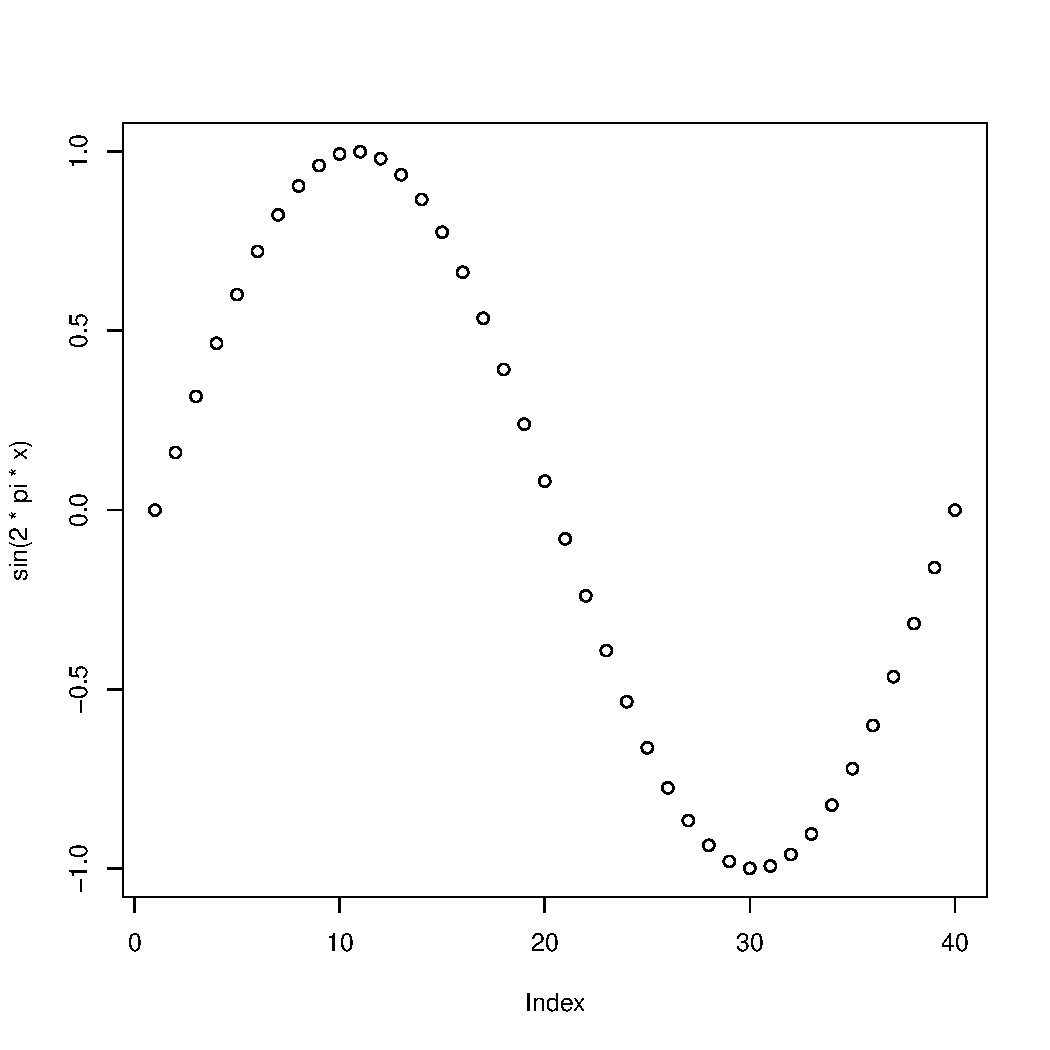
\includegraphics[width=\textwidth]{Plot_Points_Sine.pdf}
  \end{subfigure}
  \begin{subfigure}[b]{.3\linewidth}
    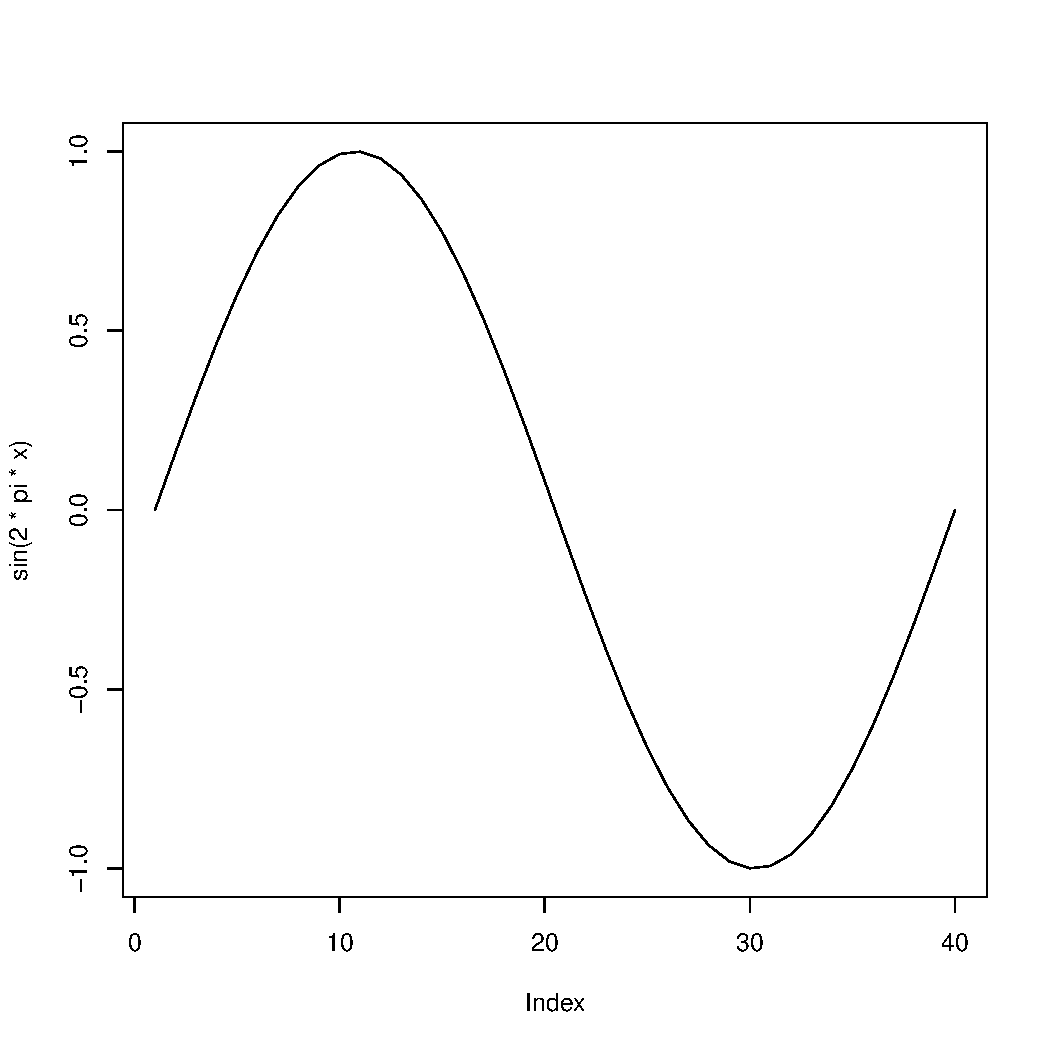
\includegraphics[width=\textwidth]{Plot_Line_Sine.pdf}
  \end{subfigure}
  \begin{subfigure}[b]{.3\linewidth}
    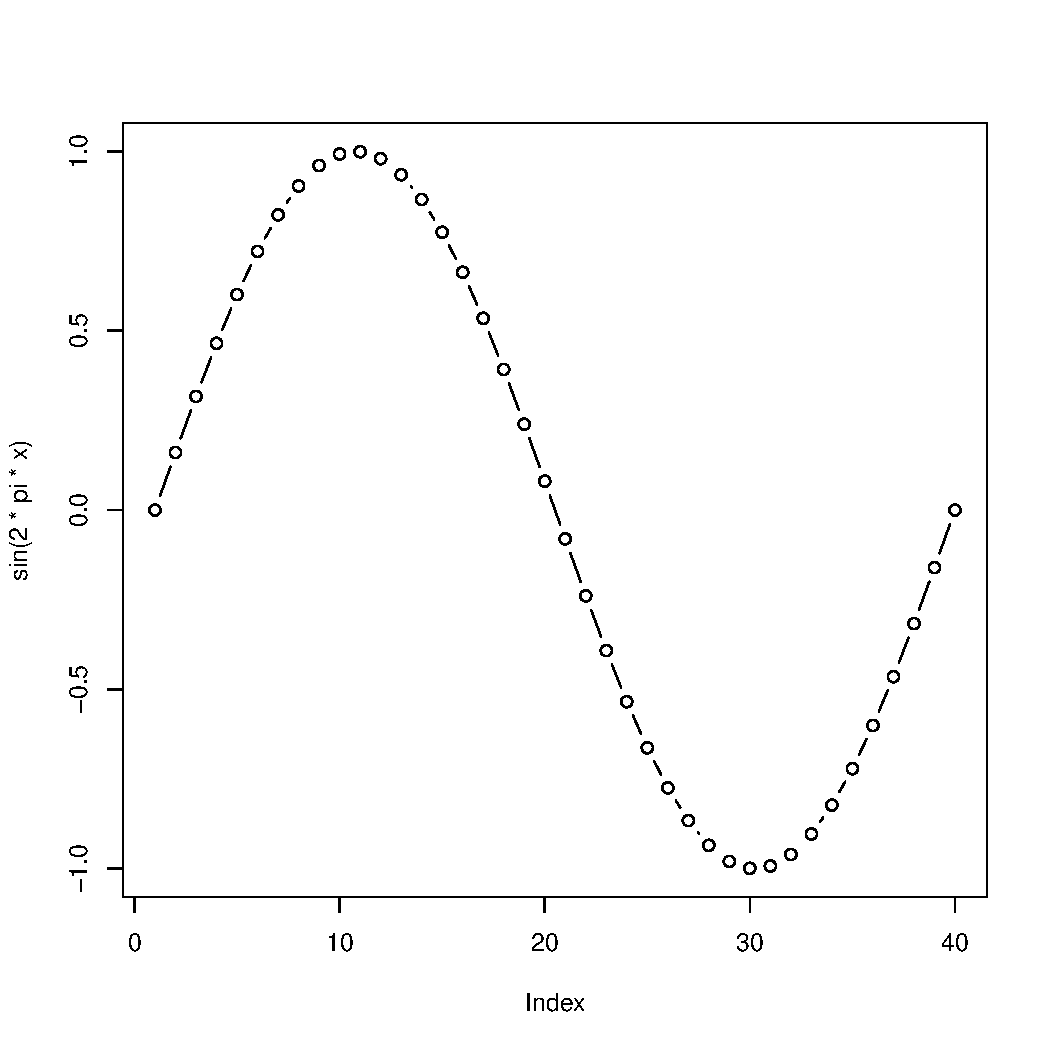
\includegraphics[width=\textwidth]{Plot_Both_Sine.pdf}
  \end{subfigure}
  \caption{Резултати од различните \mintinline{R}{plot} типови.}
\end{figure}
\end{frame}

\begin{frame}[fragile]
\begin{minted}{R}
> plot(Cars93$Weight, Cars93$EngineSize,
+      col=as.numeric(Cars93$Type),
+      pch=as.numeric(Cars93$Type))
\end{minted}
\begin{figure}
  \centering
  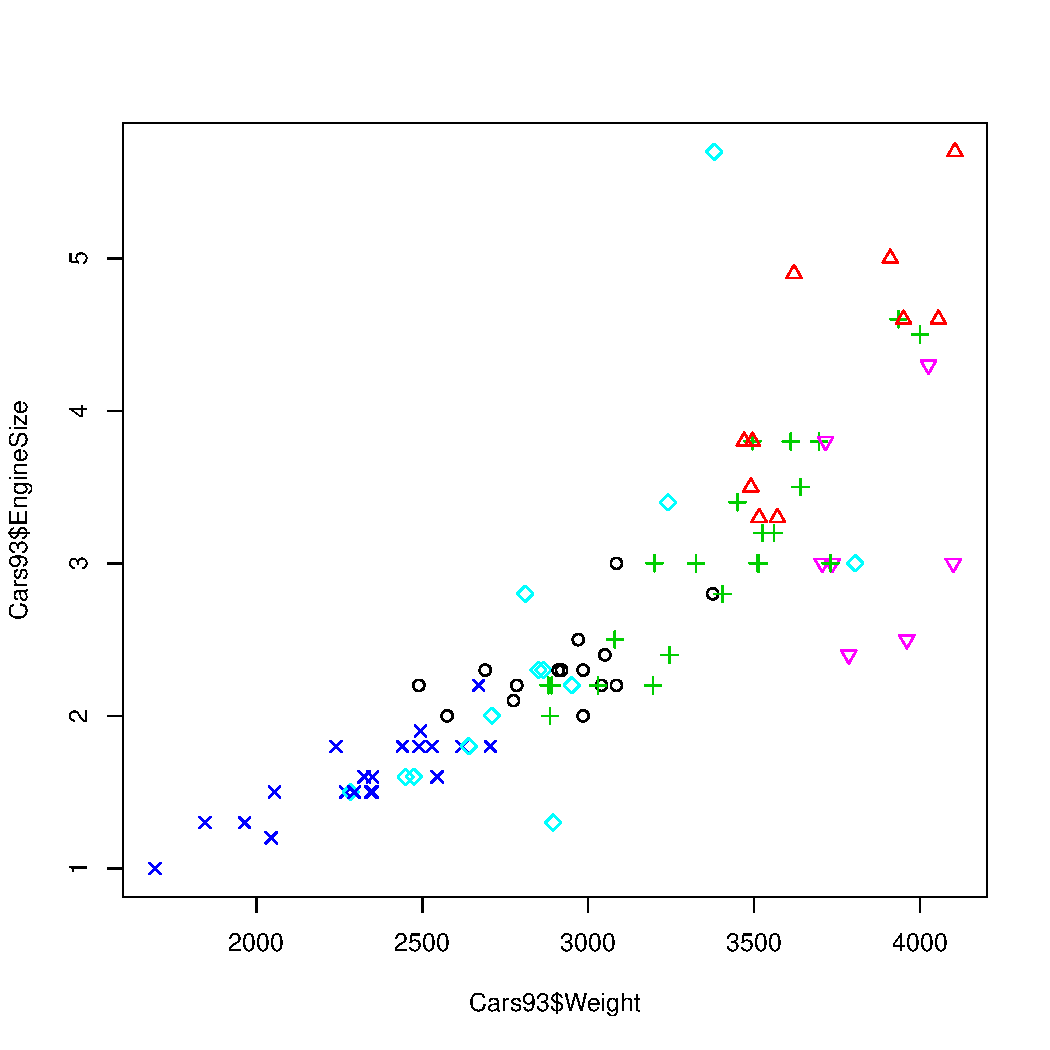
\includegraphics[width=.5\textwidth]{Plot_Cars.pdf}
  \caption{Тежина наспрема големина на мотор.}
\end{figure}
\end{frame}

\begin{frame}[fragile]{Додавање на текст, линии, легенда...}
  Постојат функции кои додаваат елементи на веќе отворен цртеж.
  \begin{itemize}
  \item \mintinline{R}{text}: додавање на текст;
  \item \mintinline{R}{legend}: додавање на легенда;
  \item \mintinline{R}{lines} и \mintinline{R}{abline}: додавање на произволни и
    прави линии соодветно;
  \item \mintinline{R}{points} и \mintinline{R}{rug}: додавање на точки односно
    rugs.
  \end{itemize}
\begin{minted}{R}
> text(max(Cars93$Weight), max(Cars93$EngineSize),
+      "maximum", pos="2")  # pos="2" значи „лево од“
> abline(v=mean(Cars93$Weight))
> abline(h=mean(Cars93$EngineSize))
> legend("topleft", legend=unique(Cars93$Type),
+        pch=unique(Cars93$Type),
+        col=unique(Cars93$Type))
\end{minted}
\end{frame}

\begin{frame}
  \begin{figure}
    \centering
    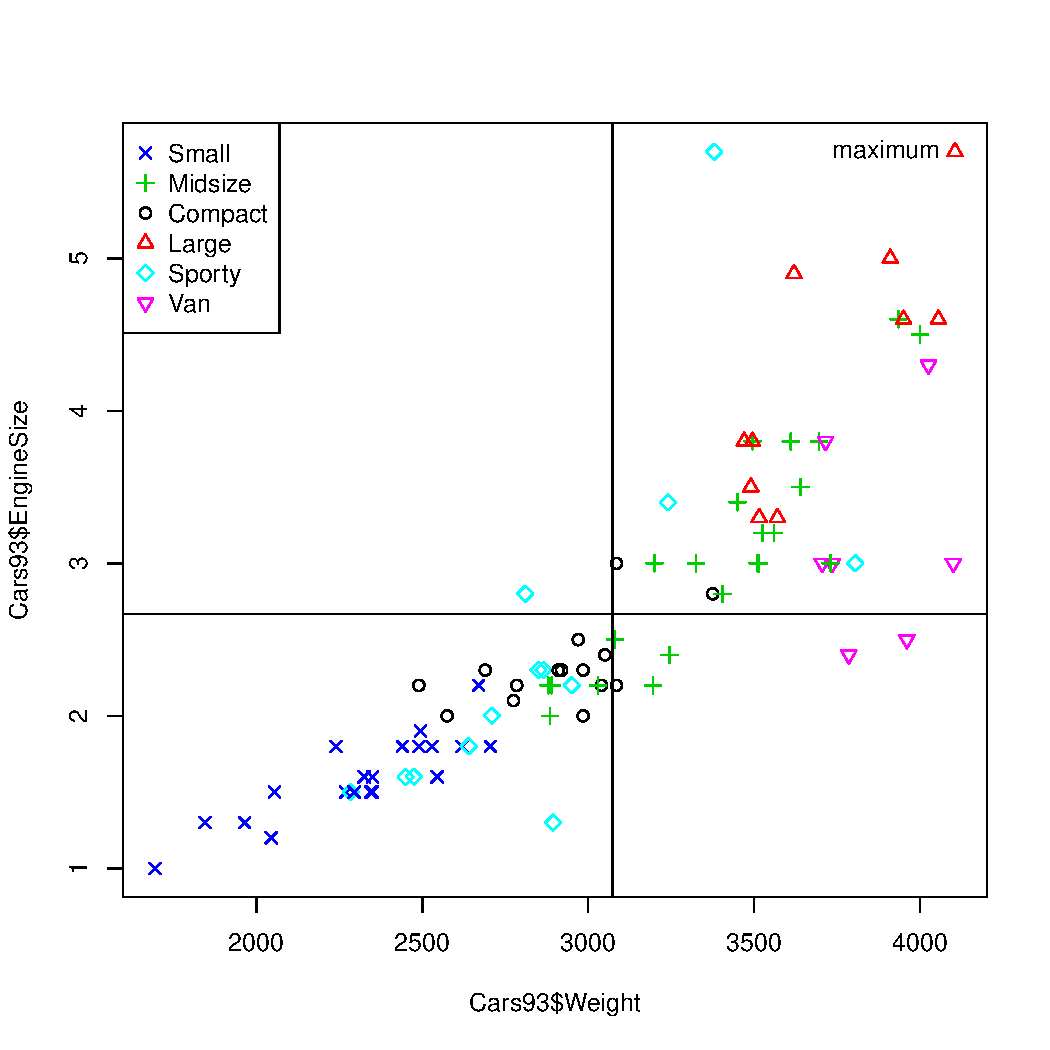
\includegraphics[width=.66\textwidth]{Plot_Cars_Decorated.pdf}
    \caption{Цртежот со додаден текст и легенда.}
  \end{figure}
\end{frame}

\begin{frame}[fragile]{Матрица од цртежи}
  Доколку \mintinline{R}{plot} ја повикаме со data frame, на сликата ќе биде
  исцртена матрица од цртежи---еден за секој пар колони.  Истото може да се
  постигне со функцијата \mintinline{R}{pairs} за произволни податоци.
\begin{minted}{R}
> plot(iris, col=iris$Species)  # или pairs(iris)
\end{minted}
  \begin{figure}
    \centering
    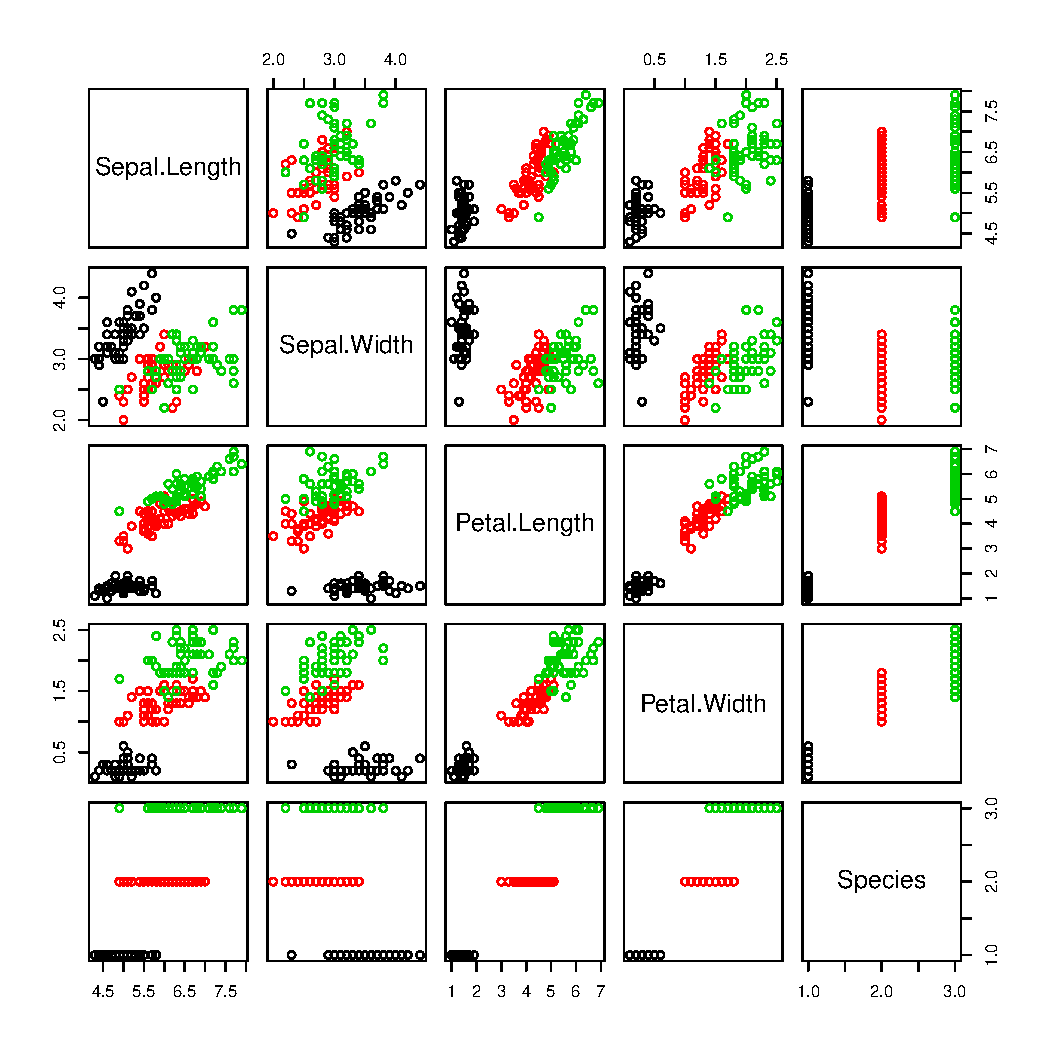
\includegraphics[width=.45\textwidth]{Plot_Pairs_Iris.pdf}
  \end{figure}
\end{frame}

\begin{frame}{Хистограми}
  Функцијата за цртање хистограми е \mintinline{R}{hist}.  Освен тоа што го црта
  хистограмот, враќа и листа со информации за него.
  \begin{itemize}
  \item \mintinline{R}{x}: вектор за кој да се направи хистограм.
  \item \mintinline{R}{breaks}: контрола на групирањето вредности:
    \begin{itemize}
    \item нумерички вектор со опсег за секоја група;
    \item број на групи (опсезите автоматски ќе бидат одредени);
    \item име на алгоритам за групирање (\mintinline{R}{"Sturges"},
      \mintinline{R}{"Scott"}, \mintinline{R}{"Freedman-Diaconis"}; default
      \mintinline{R}{"Sturges"}).
    \end{itemize}
  \item \mintinline{R}{freq}: ако е \mintinline{R}{TRUE}, се цртаат фреквенции,
    инаку се црта густина.  По default е \mintinline{R}{TRUE} кога
    \mintinline{R}{breaks} се на еднаква оддалеченост.
  \item \mintinline{R}{plot}: ако е \mintinline{R}{FALSE}, хистограмот нема да
    биде исцртан.  Кога е \mintinline{R}{TRUE}, може да се пратат дополнителни
    аргументи како \mintinline{R}{col}, \mintinline{R}{xlim},
    \mintinline{R}{ylim}, ...
  \end{itemize}
\end{frame}

\begin{frame}[fragile]{Хистограми}{Пример}
\begin{minted}[mathescape]{R}
> BMI <- rnorm(10^3, mean=24.2, sd=2.2)
> BMI.hist <- hist(BMI, freq=FALSE, xlab="Body Mass Index",
+                  main="BMI Distribution")
> lines(density(BMI), lty=2, col="red")
> sum(diff(BMI.hist$breaks) * BMI.hist$density) # $\int\nolimits_{-\infty}^{\infty} (\mathrm{hist}) \operatorname{d} x$
[1] 1
\end{minted}
  \begin{figure}
    \centering
    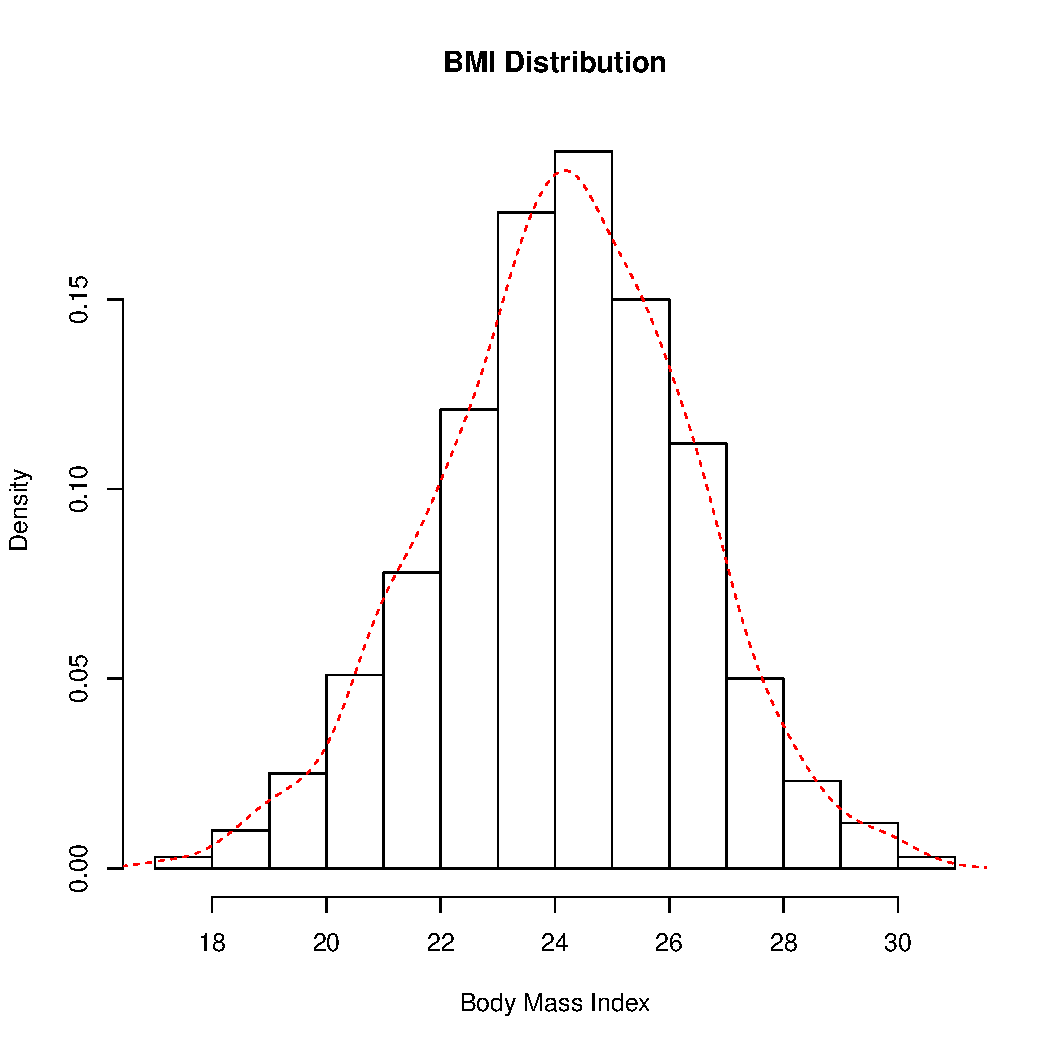
\includegraphics[width=.33\textwidth]{Histogram_BMI.pdf}
  \end{figure}
\end{frame}

\begin{frame}[fragile]{Хистограми}{Пример}
\begin{minted}{R}
> hist(Cars93$Weight,
+      breaks=c(1500, 2050, 2300, 2350, 2400, 2500,
+      3000, 3500, 3570, 4000, 4500),
+      xlab="Weight", main="Histogram of Weight")
> USA.weight <- Cars93$Weight[Cars93$Origin == "USA"]
> nonUSA.weight <- Cars93$Weight[Cars93$Origin == "non-USA"]
> hist(USA.weight, breaks=10)
> hist(nonUSA.weight, breaks=10)
\end{minted}
\end{frame}

\begin{frame}
  \begin{figure}
    \centering
    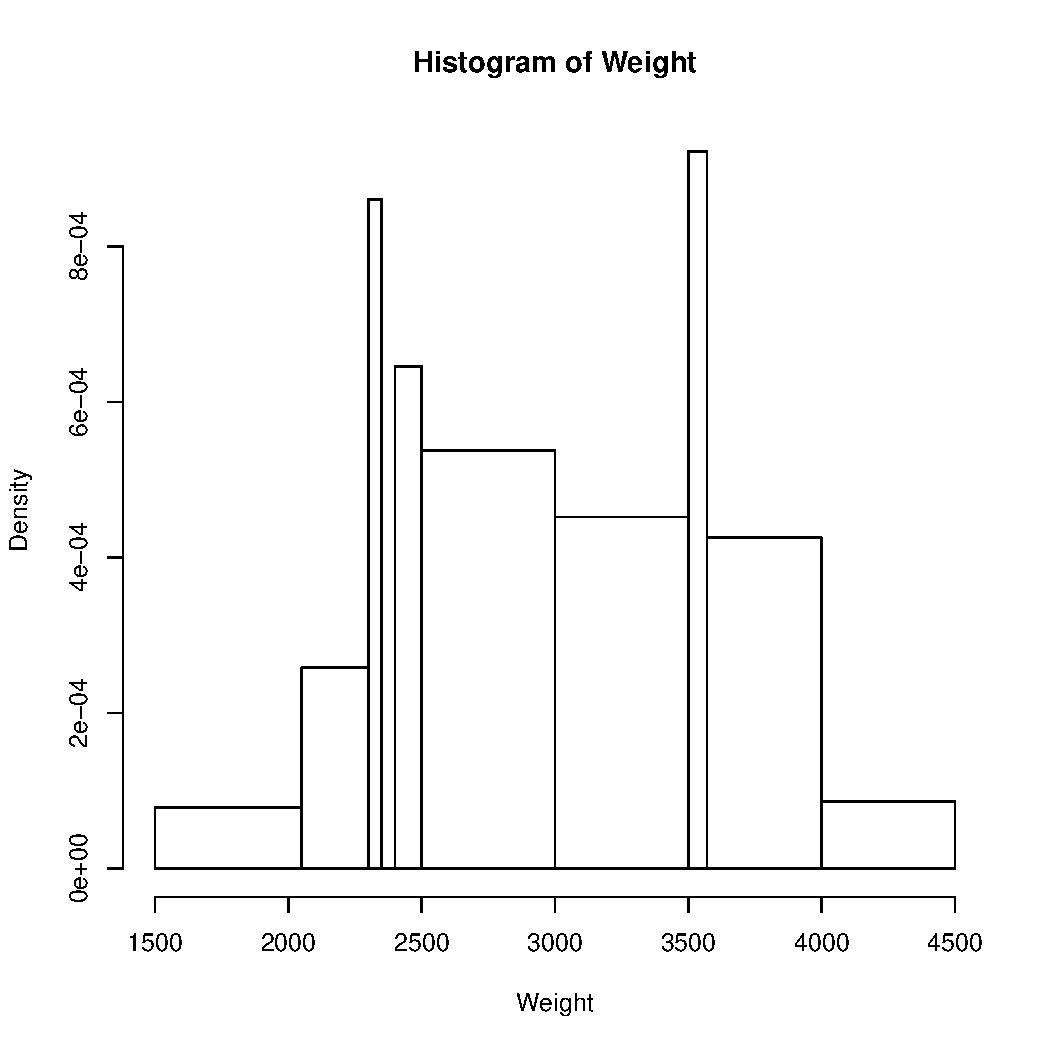
\includegraphics[width=.66\textwidth]{Histogram_Car_Weights.pdf}
    \caption{Хистограм од \mintinline{R}{Cars93$Weight}.}
  \end{figure}
\end{frame}

\begin{frame}
  \begin{figure}
    \centering
    \begin{subfigure}[b]{.45\linewidth}
      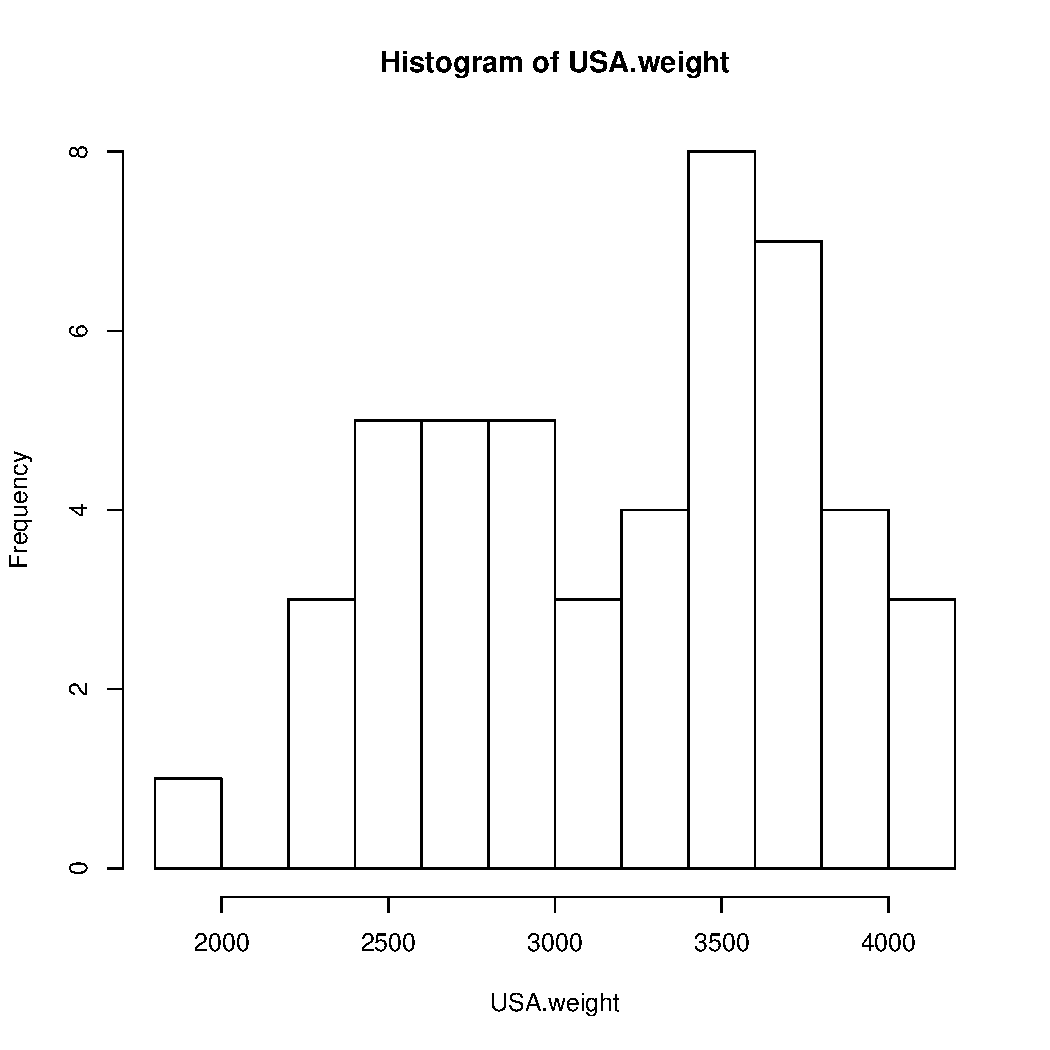
\includegraphics[width=\textwidth]{Histogram_USA_Cars.pdf}
    \end{subfigure}
    \begin{subfigure}[b]{.45\linewidth}
      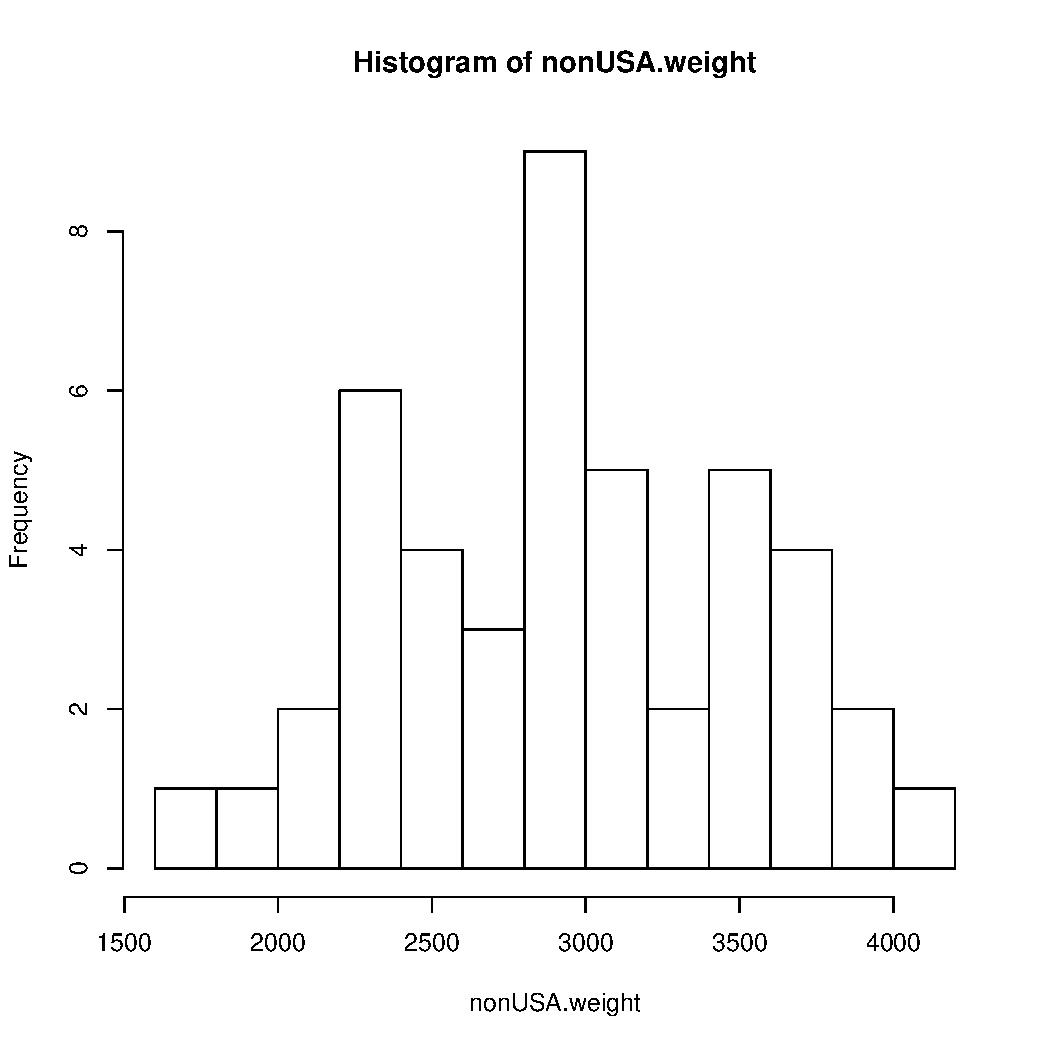
\includegraphics[width=\textwidth]{Histogram_non-USA_Cars.pdf}
    \end{subfigure}
    \caption{Тежини на автомобилите од САД и од други земји.}
  \end{figure}
\end{frame}

\begin{frame}{Boxplots}
  Boxplots се користат за графички приказ на групи преку нивните квантили.
  \begin{itemize}
  \item Освен box, секој boxplot содржи и вертикални линии (\emph{whiskers}) кои
    ја кажуваат варијабилноста во пониските квантили.
  \item Box-от го зафаќа целиот IQR, каде медијаната е означена со затемнета
    линија.
  \item Whiskers-ите се протегаат сѐ до \(1.5 \cdot \mathrm{IQR}\).
  \item Податоците надвор од \(1.5 \cdot \mathrm{IQR}\) се познати како
    \emph{outliers}.
  \end{itemize}

  Во R тие се цртаат со функцијата \mintinline{R}{boxplot}.  Таа како аргумент
  прифаќа \emph{формула}: објект од типот на \mintinline{R}{value ~ group}, што
  кажува да се нацрта boxplot за \mintinline{text}{value} за секоја вредност од
  \mintinline{text}{group}.
\end{frame}

\begin{frame}[fragile]{Boxplots}{Пример}
\begin{minted}{R}
> boxplot(len ~ supp * dose, data=ToothGrowth,
+         col=c("gold", "darkgreen"),
+         main="Tooth Growth", xlab="Supplement and Dose")
> boxplot(trees$Girth, main="Tree Girth", xlab="Girth")
\end{minted}
  \begin{figure}
    \centering
    \begin{subfigure}[b]{.45\linewidth}
      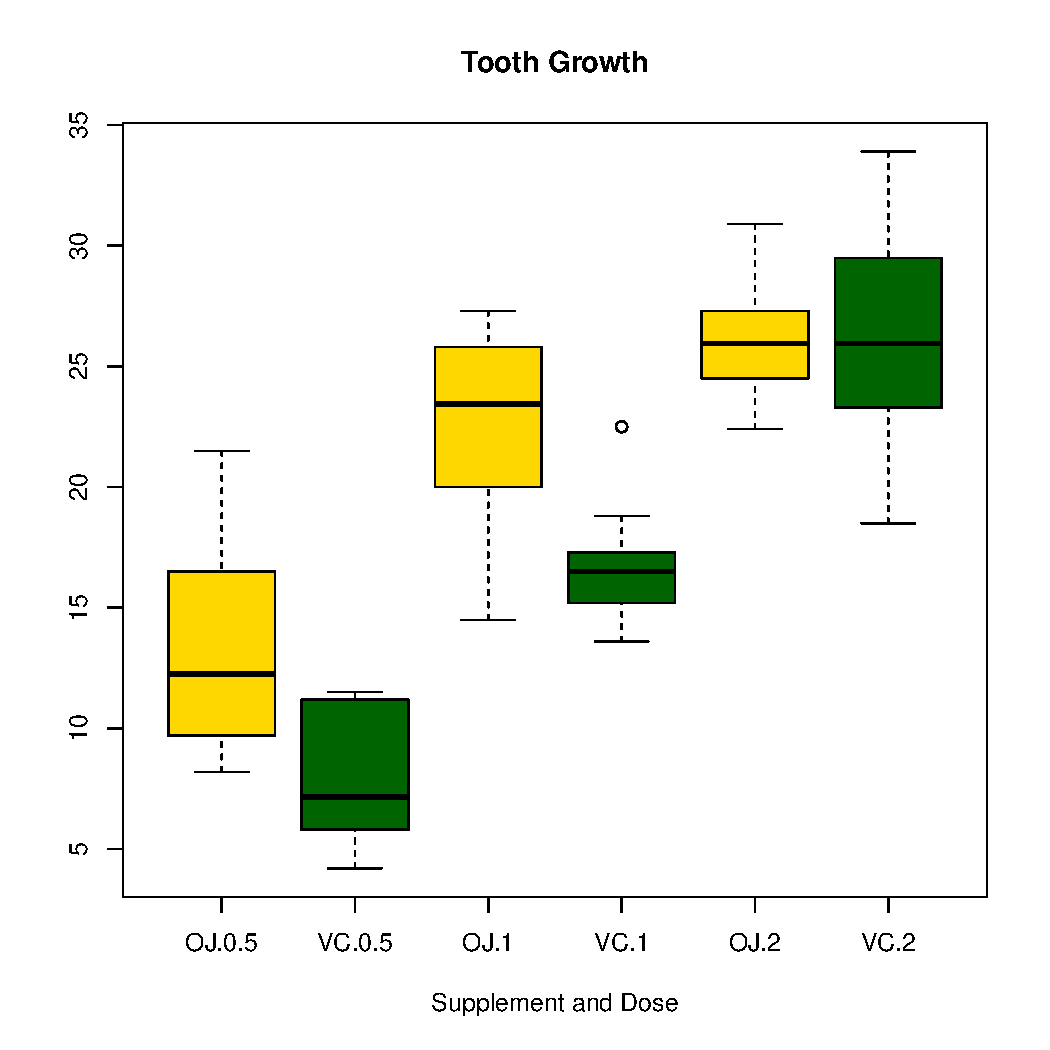
\includegraphics[width=\textwidth]{Boxplot_Tooth_Growth.pdf}
    \end{subfigure}
    \begin{subfigure}[b]{.45\linewidth}
      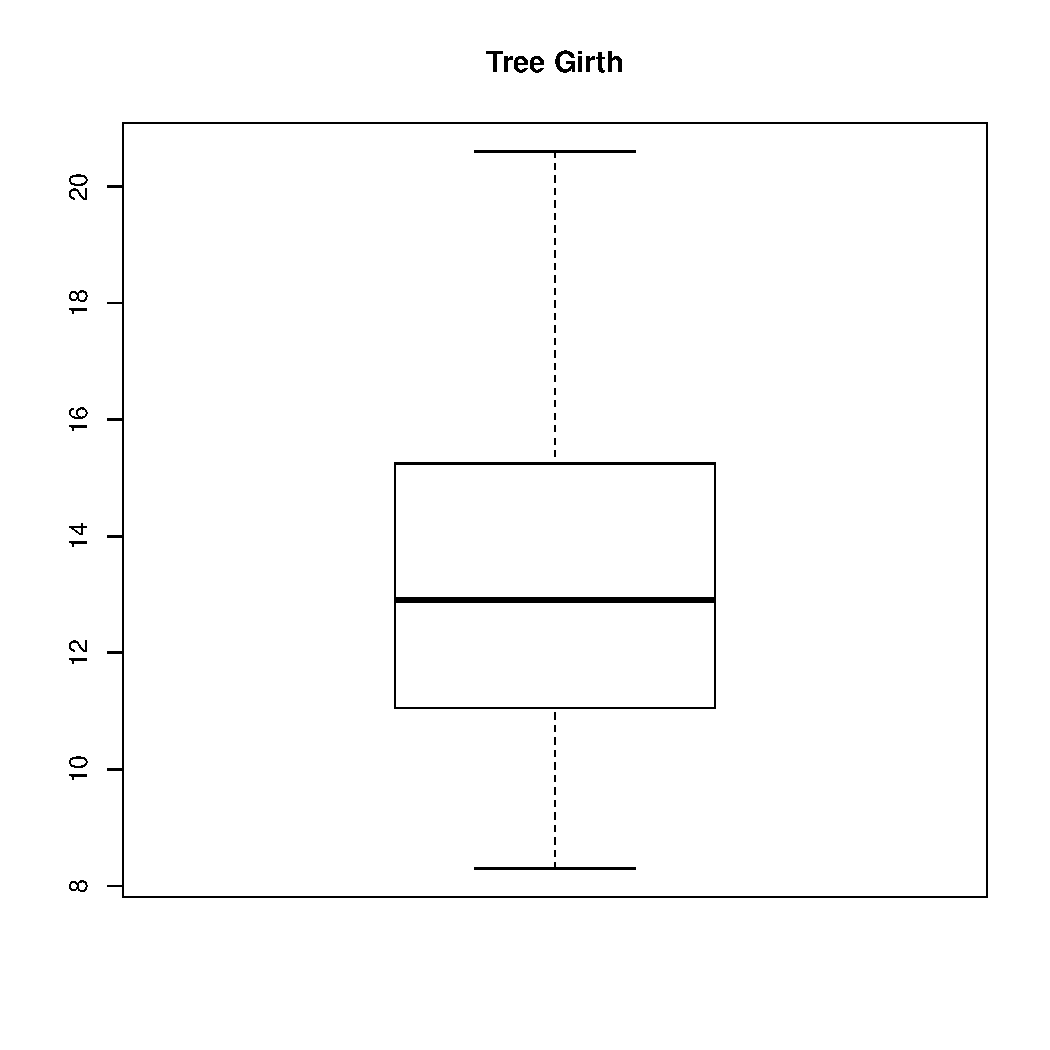
\includegraphics[width=\textwidth]{Boxplot_Tree_Girth.pdf}
    \end{subfigure}
  \end{figure}
\end{frame}

\begin{frame}{Q--Q (квантил--квантил) plot}
  Q--Q plot е метод за графичка споредба на две распределби преку споредба на
  нивните квантили.
  \begin{itemize}
  \item Една точка \((x, y)\) во Q--Q plot-от соодветствува на еден од
    квантилите на втората распределба (\(y\)-координата) наспрема истиот квантил
    од првата распределба (\(x\)-координата).
  \item Ако квантилите се слични, точките од Q--Q plot-от би лежеле близу
    линијата \(y = x\).
  \item Доколку постои линеарна зависност помеѓу распределбите, точките од Q--Q
    plot-от би лежеле на линија, но во општ случај не на \(y = x\).
  \end{itemize}

  Во R се користат функциите \mintinline{R}{qqplot}, \mintinline{R}{qqnorm}, и
  \mintinline{R}{qqline}.
\end{frame}

\begin{frame}[fragile]{Q--Q plot}{Пример}
\begin{minted}{R}
> qqplot(iris$Petal.Width, iris$Petal.Length)
> qqplot(iris$Sepal.Width, iris$Sepal.Length)
\end{minted}
  \begin{figure}
    \centering
    \begin{subfigure}[b]{.45\linewidth}
      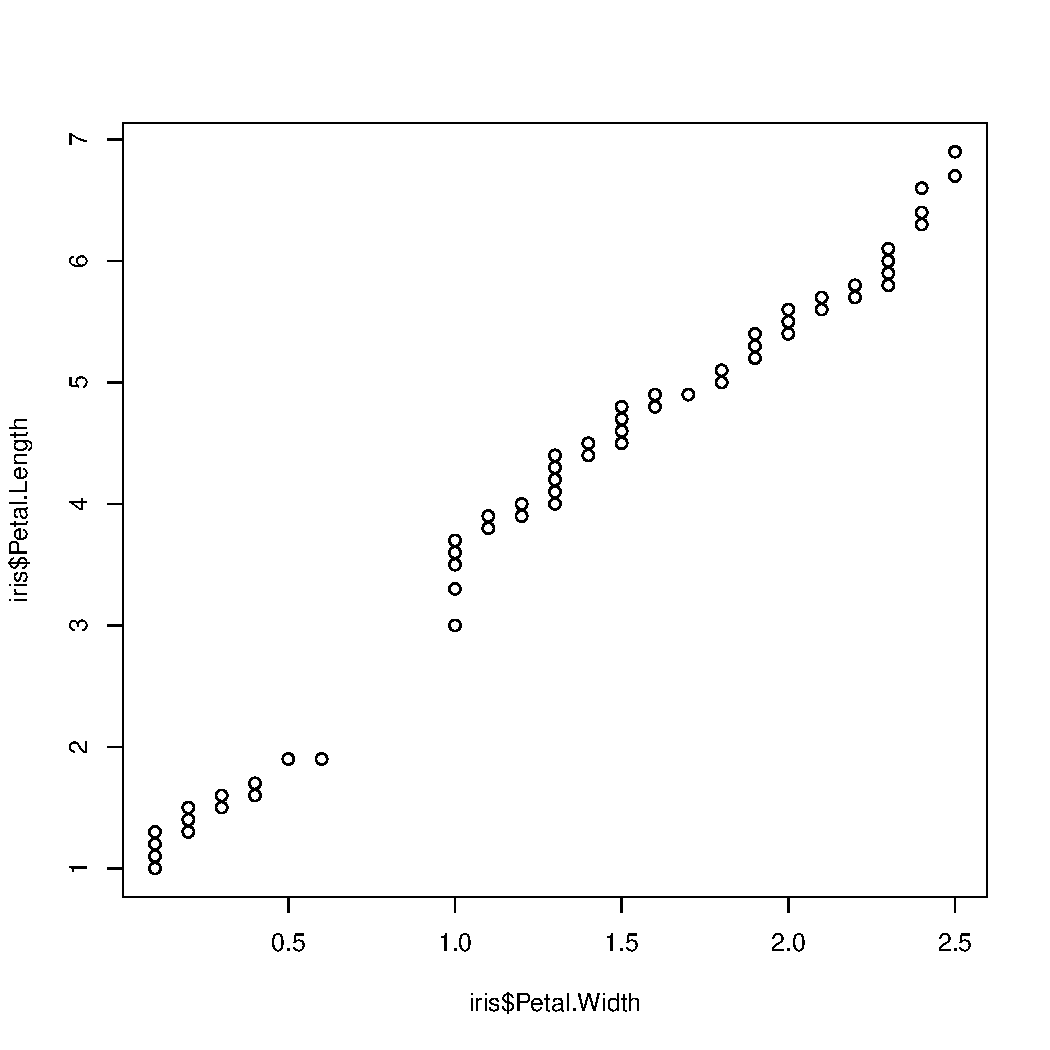
\includegraphics[width=\textwidth]{QQ_Petal_Sizes.pdf}
    \end{subfigure}
    \begin{subfigure}[b]{.45\linewidth}
      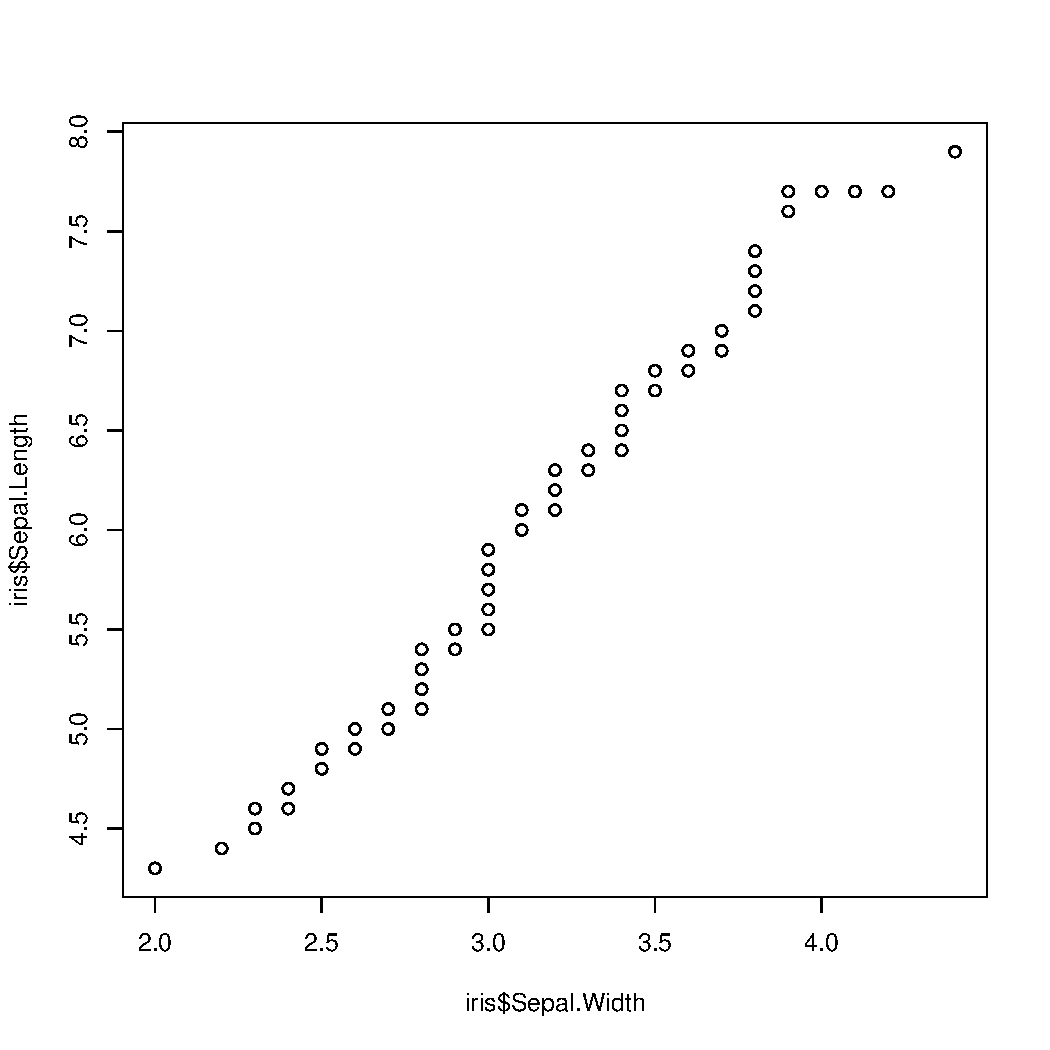
\includegraphics[width=\textwidth]{QQ_Sepal_Sizes.pdf}
    \end{subfigure}
  \end{figure}
\end{frame}

\begin{frame}[fragile]{Q--Q plot}{Пример}
\begin{minted}{R}
> qqnorm(iris$Sepal.Length)
> qqline(iris$Sepal.Length)
\end{minted}
  \begin{figure}
    \centering
    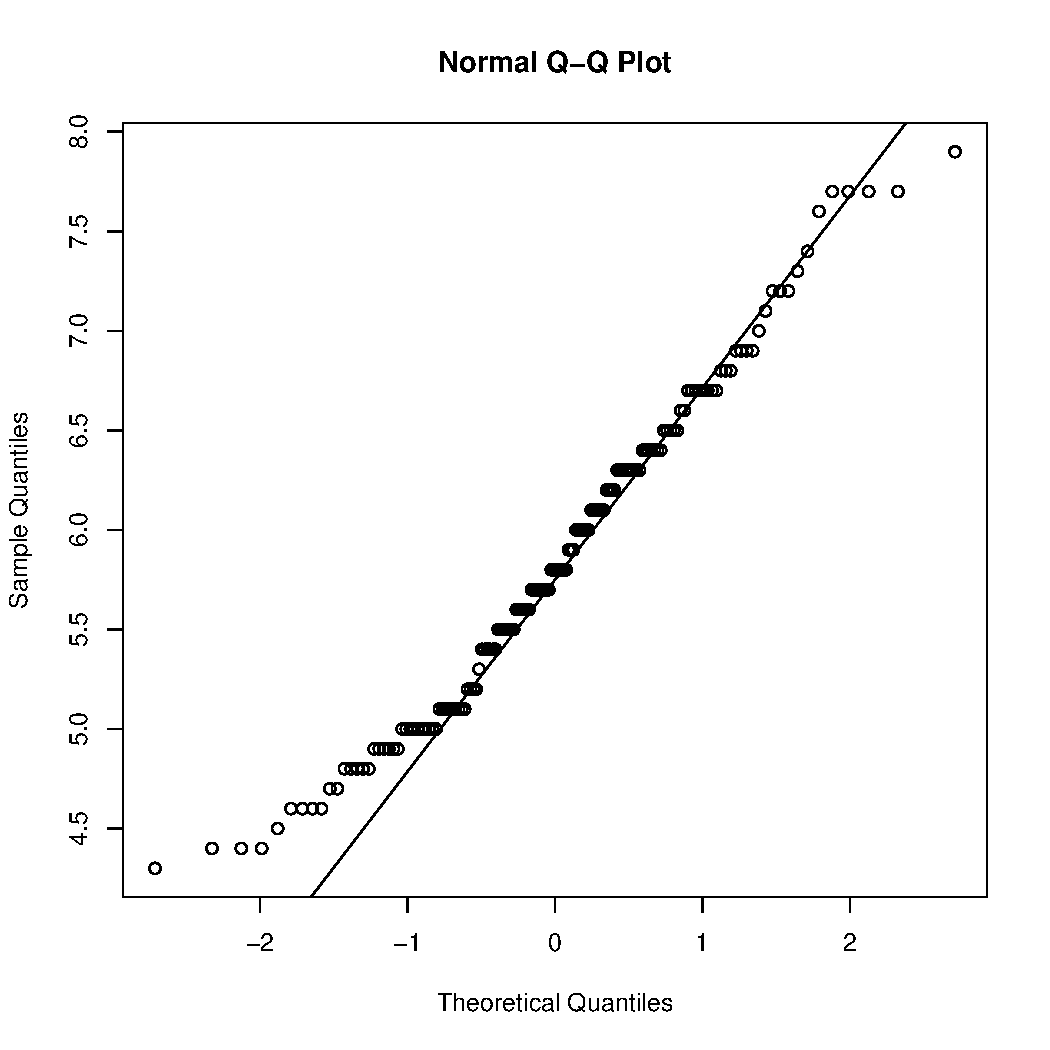
\includegraphics[width=.5\textwidth]{QQ-norm_Sepal_Length.pdf}
  \end{figure}
\end{frame}

\begin{frame}{Централна гранична теорема}
  Централната гранична теорема е една од фундаменталните теореми во
  веројатноста.  Таа, освен тоа што е од теориски интерес, наоѓа голема примена
  во статистиката.
  \begin{theorem}[Централна гранична теорема, Линдеберг--Леви]
    Нека \((X_1, X_2, \ldots, X_n)\) биде случаен примерок од обележје \(X\) со
    средна вредност \(\mu\) и варијанса \(\sigma^2 < \infty\).  Тогаш
    \[
      \sqrt{\frac{n}{\sigma^2}} \left(\left(\frac{\sum\nolimits_{k = 1}^{n}
            X_i}{n}\right) - \mu\right) \xrightarrow{d}
      \operatorname{\mathcal{N}}(0, 1)\text{,}
    \]
    каде \(\xrightarrow{d}\) означува \emph{конвергенција во распределба}.
  \end{theorem}
\end{frame}

\begin{frame}[fragile]{Централна гранична теорема}{Илустрација}
  За да ја илустрираме централната гранична теорема, ќе ја исцртаме
  распределбата на стандардизираната средна вредност од сто
  \(\operatorname{\mathcal{U}}(0, 1)\) случајни променливи.
\begin{minted}{R}
> m <- 10^4
> n <- 100
> X <- matrix(runif(m * n), nrow=m)
> X.norm <- (apply(X, 1, sum) - 0.5 * n) / sqrt(n / 12)
> # Верификација со хистограм
> hist(X.norm, freq=FALSE)
> curve(dnorm(x), add=TRUE)
> # Верификација со Q-Q plot
> qqnorm(X.norm)
> qqline(X.norm)
\end{minted}
\end{frame}

\begin{frame}{Централна гранична теорема}{Илустрација}
  \begin{figure}
    \centering
    \begin{subfigure}[b]{.45\linewidth}
      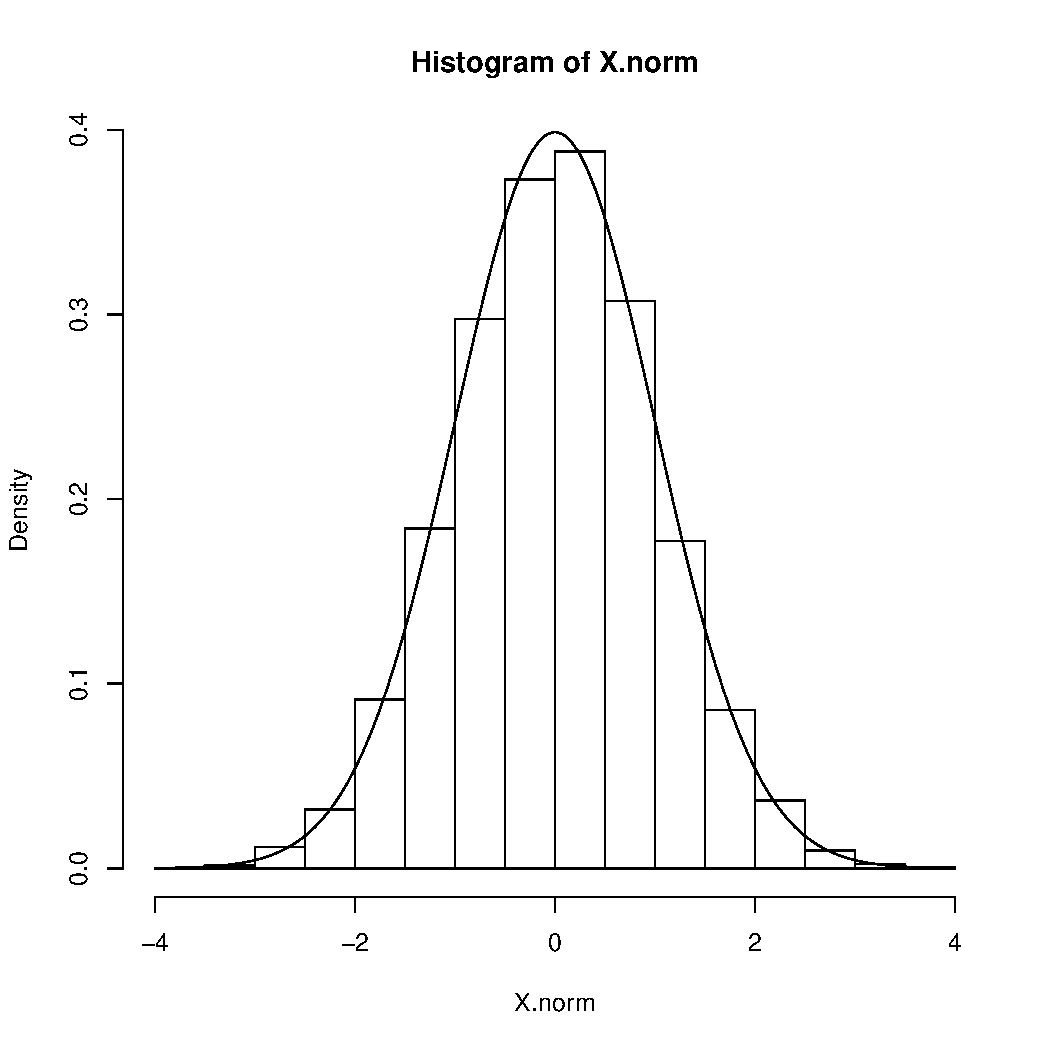
\includegraphics[width=\textwidth]{Histogram_CLT.pdf}
    \end{subfigure}
    \begin{subfigure}[b]{.45\linewidth}
      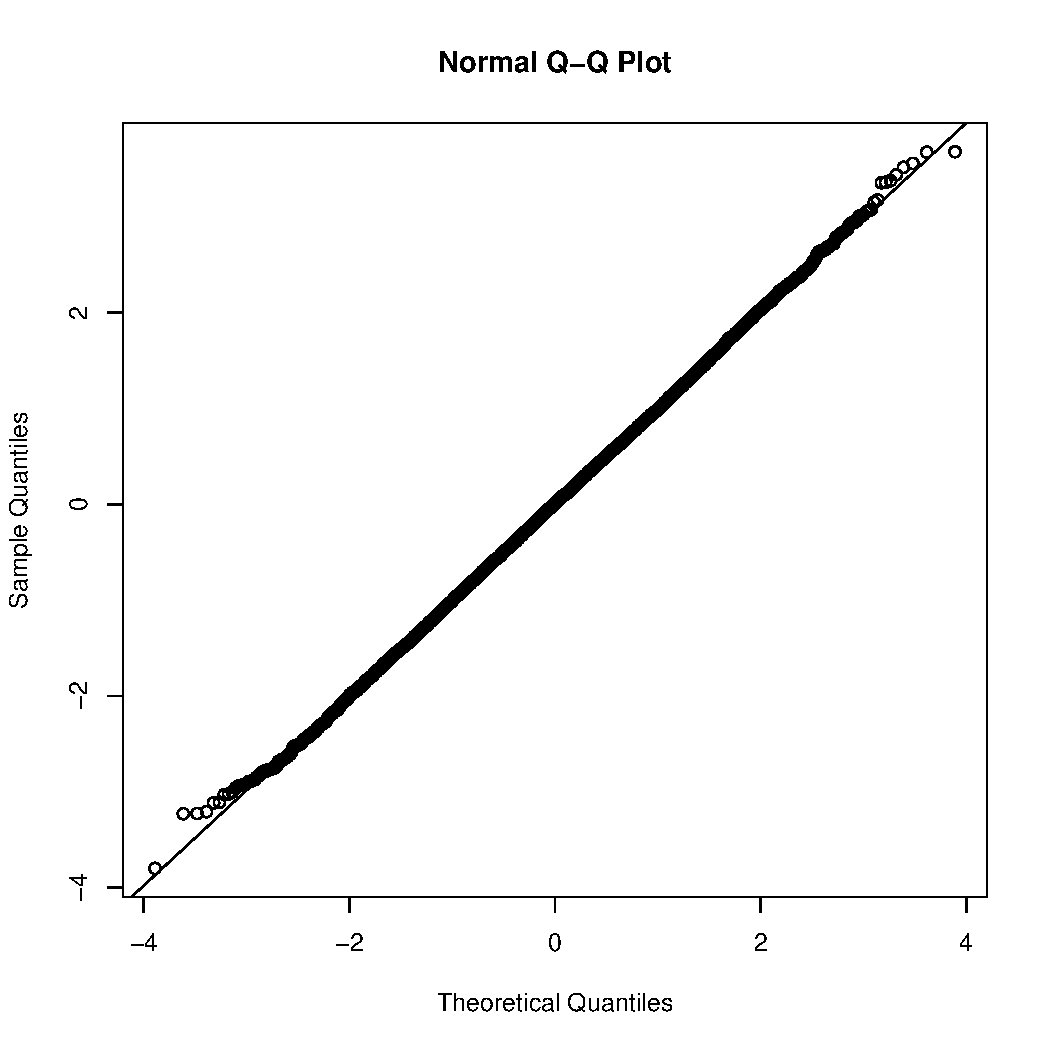
\includegraphics[width=\textwidth]{QQ_CLT.pdf}
    \end{subfigure}
    \caption{Верификација на централната гранична теорема.}
  \end{figure}
\end{frame}

\section{Оценување на параметри}

\begin{frame}{Метод на моменти}
  Методот на моменти врши оценување на параметрите на една распределба преку
  изедначување на теориските со моментите на примерокот.
  \begin{definition}[Метод на моменти]
    Нека \((X_1, X_2, \ldots, X_n)\) е случаен примерок од обележје \(X\) чија
    распределба зависи од параметри \(\theta_1, \theta_2, \ldots, \theta_m\).
    Оценувачи по метод на моменти
    \(\hat{\theta}_1, \hat{\theta}_2, \ldots, \hat{\theta}_m\) се добиваат така
    што \(m\) теориски моменти од распределбата на \(X\) ќе се изедначат со
    истите \(m\) моменти на примерокот, и равенките ќе се решат по непознатите
    параметри.
  \end{definition}
\end{frame}

\begin{frame}[fragile]{Метод на моменти}{Пример во R}
  Веќе ги имаме разработено сите потребни функции за методот на моменти да го
  примениме во R.  На пример, знаеме дека ако
  \(X \sim \operatorname{Pois}(\lambda)\), тогаш
  \(\operatorname{\mathbb{E}}[X] = \lambda\) и
  \(\operatorname{\mathbb{D}}[X] = \lambda\).  Оттука добиваме
  \begin{align*}
    \hat{\lambda} &= \bar{X}\text{, или}\\
    \hat{\lambda} &= S^2\text{.}
  \end{align*}
\begin{minted}{R}
> lambda <- 5
> x <- rpois(10^5, lambda)
> mean(x)
[1] 5.00487
> var(x)
[1] 5.002956
\end{minted}
\end{frame}

\begin{frame}[fragile]{Метод на моменти}{Пример во R}
  Ако \(X \sim \operatorname{\mathcal{N}}(\mu, \sigma^2)\), добиваме дека
  \begin{align*}
    \hat{\mu} &= \bar{X} \\
    \hat{\sigma}^2 &= \frac{n - 1}{n} S^2\text{.}
  \end{align*}
\begin{minted}[mathescape]{R}
> n <- 10^4
> mu <- 5; sd <- 2  # $\mu = 5$, $\sigma^2 = 4$
> x <- rnorm(n, mu, sd)
> mean(x)
[1] 4.994426
> (n - 1) / n * var(x)
[1] 3.942171
\end{minted}
\end{frame}

\begin{frame}{Метод на маскимална подобност}
  Методот на максимална подобност е специјален случај на \emph{максимум а
    постериори} оценувач кој го наоѓа параметарот кој ја максимизира подобноста
  на дадената реализација на примерокот.
  \begin{definition}[Метод на максимална подобност]
    Нека \((x_1, x_2, \ldots, x_n)\) биде реализација на случајниот примерок
    \((X_1, X_2, \ldots, X_n)\) од обележјето \(X\).  Распределбата на \(X\)
    припаѓа на фамилија распределби
    \(\{p(\cdot \mid \theta) : \theta \in \Theta\}\).  Ако ги фиксираме
    \((x_1, x_2, \ldots, x_n)\), и \(p(x_1, x_2, \ldots, x_n \mid \theta)\) ја
    гледаме како функција од \(\theta\),
    \(\mathcal{L}(\theta \mid x_1, x_2, \ldots, x_n)\), тогаш оценувач за
    \(\theta\) по методот на максимална подобност е
    \[
      \hat{\theta} = \argmax_{\theta \in \Theta} \mathcal{L}(\theta \mid x_1,
      x_2, \ldots, x_n)\text{.}
    \]
  \end{definition}
\end{frame}

\begin{frame}{Метод на максимална подобност}
  Бидејќи случајниот примерок се состои од независни и идентично распределени
  случајни променливи,
  \[
    \mathcal{L}(\theta \mid x_1, x_2, \ldots, x_n) = p(x_1, x_2, \ldots, x_n
    \mid \theta) = \prod\limits_{k = 1}^{n} p(x_k \mid \theta)\text{.}
  \]

  Често е поедноставно да се максимизира
  \[
    \ln \mathcal{L}(\theta \mid x_1, x_2, \ldots, x_n) = \sum\limits_{k = 1}^{n}
    \ln p(x_k \mid \theta)\text{.}
  \]

  Оценувачите добиени по методот на максимална подобност поседуваат добри
  статистички својства и се често користени во пракса.
\end{frame}

\begin{frame}[fragile]{Метод на максимална подобност}{Пример}
  Во R, ќе ја користиме функцијата \mintinline{R}{mle} од библиотеката
  \mintinline{R}{stats4}.  Од нас единствено се бара да дефинираме функција која
  ќе пресметува \(-\ln \mathcal{L}(\theta \mid x_1, x_2, \ldots, x_n)\) (да го
  забележиме минусот напред).  Доколку имаме примерок од експоненцијална
  распределба:
\begin{minted}[mathescape]{R}
> library(stats4)
> x <- rexp(10^4, rate=3)
> nll <- function(lambda=0.1) {
+   -sum(dexp(x, rate=lambda, log=TRUE))  # $-\sum\nolimits_{k = 1}^{n} \ln p(x_k \mid \lambda)$.
+ }
> mle(nll)
Coefficients:
  lambda
3.075704
\end{minted}
\end{frame}

\begin{frame}[fragile]{Метод на максимална подобност}{Пример}
  Функцијата \mintinline{R}{mle} врши нумеричка оптимизација на дефинираната од
  нас функција \mintinline{R}{nll} и го враќа минимумот.
  \begin{itemize}
  \item Потребна е почетна вредност за параметрите, која може да биде зададена
    во дефиницијата на функцијата или преку аргументот \mintinline{R}{start}.
  \item Најчесто, почетната вредност не игра никаква улога.
  \end{itemize}
\begin{minted}{R}
> y <- rgamma(10^4, shape=3, rate=2)
> nll <- function(shape, rate) {
+   -sum(dgamma(y, shape, rate, log=TRUE))
+ }
> mle(nll, start=list(shape=1, rate=1))
Coefficients:
   shape     rate
3.013568 2.013409
\end{minted}
\end{frame}

\end{document}

%%% Local Variables:
%%% mode: latex
%%% fill-column: 80
%%% TeX-command-extra-options: "-shell-escape"
%%% TeX-master: t
%%% End: